\documentclass[spanish,a4paper,14pt,oneside]{extreport}

\usepackage[utf8]{inputenc}
\usepackage[spanish]{babel}
\usepackage[pdftex]{graphicx}
\usepackage{hyperref}
\usepackage{url}
\graphicspath{{Imagenes/}}
\usepackage{listings}
\usepackage{color}

%\usepackage{biblatex}
%\usepackage[dvips]{graphicx}
%\usepackage[dvips]{epsfig}
%\usepackage{alltt}
%\usepackage{algorithm}
%\usepackage{algorithmic}
%\usepackage{multirow}
%\usepackage[top=2cm, bottom=2cm, left=2cm, right=2cm]{geometry}

%Evitar partir palabras al final de la línea
\hyphenpenalty=10000
\tolerance=1000

%%%%%%%%%%%%%%ESTILO PARA CÓDIGO%%%%%%%%%%%%%%%%%%%%%%%%%%%%%%%%%%%%%%%
\definecolor{violet}{rgb}{0.5,0,0.5}
\definecolor{navy}{rgb}{0,0,0.5}
\definecolor{hellgelb}{rgb}{0.95,0.95,0.92}
\definecolor{colKeys}{rgb}{0,0,1}
\definecolor{colIdentifier}{rgb}{0,0,0}
\definecolor{colComments}{rgb}{1,0,0}
\definecolor{colString}{rgb}{0,0.5,0}

\lstset{
	float=htbp,
	language = Java,
	basicstyle=\ttfamily\small,
	identifierstyle=\color{colIdentifier},
	keywordstyle=\color{colKeys},
	stringstyle=\color{colString},
	commentstyle=\color{colComments},
	columns=flexible,
	tabsize=3,
	frame=single,
	extendedchars=true,
	showspaces=false,
	showstringspaces=false,
	numbers=left,
	numberstyle=\tiny,
	breaklines=true,
	backgroundcolor=\color{hellgelb},
	breakautoindent=true,
	captionpos=b,
	breakatwhitespace=true,
	aboveskip=10pt,
	belowskip=10pt,
}

\renewcommand{\lstlistingname}{Listado} % Los títulos de los códigos insertados se denotan con Listado...
%\renewcommand{\lstlistingname}{Ejemplo} % Los títulos de los códigos insertados se denotan con Ejemplo...

%%%%%%%%%%%%%%%%%%%%%%%%%%%%%%%%%%%%%%%%%%%%%%%%%%%%%%%%%%%%%%%%%%%%%%%%%%%%%%%%%%%%%%%%%%%%%%%%
\newcommand{\CollegeApp}{\texttt{SchoolApp }{}}
\newcommand{\workTitle}{\texttt{SchoolApp: Comunicación desde las aulas.}{}}
\newcommand{\englishWorkTitle}{\texttt{``SchoolApp'': Comunication from the classroom.}{}}

\newenvironment{summary}{
	\par
	\noindent
	\begin{center}
		\textbf{Abstract}
	\end{center}
	\begin{itshape}
		\par
		\noindent
	\end{itshape}}
	
%%%%%%%%%%%%%%%%%%%%%%%%%%%%%%%%%%%%%%%%%%%%%%%%%%%%%%%%%%%%%%%%%%%%%%%%%%%%%%%%%%%%%%%%%%%%%%%%

\begin{document}
	%%%%%%Capitulos definitivos%%%%%%
	%
% ---------------------------------------------------
%
% Trabajo de Final de Grado:
% Author: Gonzalo Jesús García Martín <dracoyue@gmail.com>
% Capítulo: Portada
% Fichero: Portada.tex
%
% ----------------------------------------------------
%

\pagestyle{empty}
\thispagestyle{empty}


\newcommand{\HRule}{\rule{\linewidth}{1mm}}
\setlength{\parindent}{0mm}
\setlength{\parskip}{0mm}

\vspace*{\stretch{0.5}}

\begin{center}

\includegraphics[scale=0.8]{Imagenes/logo_vertical}\\[10mm]
{\Huge Trabajo de Fin de Grado}
\end{center}

\HRule
\begin{flushright}
        {\Huge Título} \\[2.5mm]
        {\Large \textit{Title in English} .} \\[5mm]
        {\Large Gonzalo J. García Martín} \\[5mm]


\end{flushright}
\HRule
\vspace*{\stretch{2}}
\begin{center}
  \Large La Laguna, \today
\end{center}

\setlength{\parindent}{5mm} %Listo
	%
% ---------------------------------------------------
%
% Trabajo de Final de Grado:
% Author: Gonzalo Jesús García Martín <dracoyue@gmail.com>
% Capítulo: Certificado
% Fichero: Certificado.tex
%
% ----------------------------------------------------
%

\newpage
%\cleardoublepage
\thispagestyle{empty}

D. {\bf Francisco de Sande González}, con DNI número 42067050--G
profesor Titular de Universidad adscrito al Departamento de Ingeniería Informática y de Sistemas
de la Universidad de La Laguna, como tutor

\bigskip
\bigskip
{\bf C E R T I F I C A}

\bigskip
\bigskip
\bigskip
Que la presente memoria titulada:

\bigskip
``{\it Título del Trabajo.}''

\bigskip
\bigskip
\bigskip

\noindent ha sido realizada bajo su dirección por D. {\bf Gonzalo J. García Martín},
con N.I.F. 78.628.877-K.

\bigskip
\bigskip

Y para que así conste, en cumplimiento de la legislación vigente y a los efectos
oportunos firman la presente en La Laguna a \today

%\cleardoublepage
%\newpage
 %Listo
	%
% ---------------------------------------------------
%
% Trabajo de Final de Grado:
% Author: Gonzalo Jesús García Martín <dracoyue@gmail.com>
% Capítulo: Agradecimientos
% Fichero: Agradecimientos.tex
%
% ----------------------------------------------------
%

\thispagestyle{empty}

{\flushright

	\begin{LARGE}
		Agradecimientos
	\end{LARGE}

	\hspace{3mm}

	\begin{large}

		\hspace{3mm}
		XXX
	
		\hspace{3mm}
		XXX
	
		\hspace{3mm}
		XXX
	
		\hspace{3mm}
		XXX

	\end{large}

} %Listo
	\newpage

\begin{huge}
Licencia
\end{huge}

\bigskip
* Si NO quiere permitir que se compartan las adaptaciones de tu obra
y NO quieres permitir usos comerciales de tu obra indica:

\begin{center}
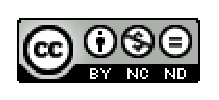
\includegraphics[scale=1.5]{Imagenes/Licencias/by-nc-nd_88x31}\\[10mm]
{\Large \copyright~Esta obra está bajo una licencia de Creative Commons Reconocimiento-NoComercial-SinObraDerivada 4.0 Internacional.
}
\end{center}


\bigskip
* Si quiere permitir que se compartan las adaptaciones de tu obra mientras se comparta de la misma manera
y NO quieres permitir usos comerciales de tu obra indica:

\begin{center}

\includegraphics[scale=1.5]{Imagenes/Licencias/by-nc-sa_88x31}\\[10mm]
{\Large \copyright~Esta obra está bajo una licencia de Creative Commons Reconocimiento-NoComercial-CompartirIgual 4.0 Internacional.
}
\end{center}



\bigskip
* Si quiere permitir que se compartan las adaptaciones de tu obra
y NO quieres permitir usos comerciales de tu obra indica:

\begin{center}

\includegraphics[scale=1.5]{Imagenes/Licencias/by-nc_88x31}\\[10mm]
{\Large \copyright~Esta obra está bajo una licencia de Creative Commons Reconocimiento-NoComercial 4.0 Internacional.
}
\end{center}

\newpage

\bigskip
*Si NO quiere permitir que se compartan las adaptaciones de tu obra
y quieres permitir usos comerciales de tu obra indica:

\begin{center}
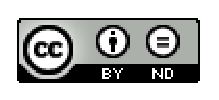
\includegraphics[scale=1.5]{Imagenes/Licencias/by-nd_88x31}\\[10mm]
{\Large \copyright~Esta obra está bajo una licencia de Creative Commons Reconocimiento-SinObraDerivada 4.0 Internacional.
}
\end{center}


\bigskip
* Si quiere permitir que se compartan las adaptaciones de tu obra mientras se comparta de la misma manera
y quieres permitir usos comerciales de tu obra (licencia de Cultura Libre) indica:

\begin{center}

\includegraphics[scale=1.5]{Imagenes/Licencias/by-sa_88x31}\\[10mm]
{\Large \copyright~Esta obra está bajo una licencia de Creative Commons Reconocimiento-CompartirIgual 4.0 Internacional.
}
\end{center}


\bigskip
* Si quiere permitir que se compartan las adaptaciones de tu obra
y quieres permitir usos comerciales de tu obra (licencia de Cultura Libre) indica:

\begin{center}

\includegraphics[scale=1.5]{Imagenes/Licencias/by_88x31}\\[10mm]
{\Large \copyright~Esta obra está bajo una licencia de Creative Commons Reconocimiento 4.0 Internacional.
}
\end{center}
 %Listo
	%
% ---------------------------------------------------
%
% Trabajo de Final de Grado:
% Author: Gonzalo Jesús García Martín <dracoyue@gmail.com>
% Capítulo: Resumen
% Fichero: Resumen.tex
%
% ----------------------------------------------------
%

\newpage  %\cleardoublepage
\begin{abstract}
	{\em
		%\bigskip
		El objetivo general de este proyecto ha sido crear una aplicación para \textit{Android} usando las nuevas tecnologías y los servicios de almacenamiento en internet, comúnmente conocidos como nube. Se pretende establecer un sistema de comunicación escolar para que los padres, madres, tutores legales, profesores y alumnos estén comunicados entre sí, intentando suplir una carencia en las aulas.
	}
\end{abstract} %A mandar
	%
% ---------------------------------------------------
%
% Trabajo de Final de Grado:
% Author: Gonzalo Jesús García Martín <dracoyue@gmail.com>
% Capítulo: Summary
% Fichero: Summary.tex
%
% ----------------------------------------------------
%

\newpage  %\cleardoublepage
\begin{summary}
	{\em
		%\bigskip
		The overall objective of this project was to create an \textit{Android} application using new technologies and the Internet storage services, commonly known as cloud. It was intended to establish a system of school communication for parents, guardians, teachers and students are interconnected.
		
		\bigskip
		With the use of these technologies has increased the number of school problems. It's not just those originating inside the classrooms and teachers can control, but also they have spread to affect students in other areas.
		
		\bigskip
		On this basis, and with the knowledge acquired throughout the Degree in Computer Engineering from the University of La Laguna, it has designed an application that can assist in academia.
		
		\bigskip
		For this we used the integrated development environment, AndroidStudio, along with Firebase, a provider of cloud services.
		
		\bigskip
		{\bf Keywords:} Android applications, mobile devices, schools, education, communication tools.
	}
\end{summary}
 %A mandar
	
	%%%%%%%%%%Numeracion en romanos%%%%%%%%%%
	\renewcommand{\thepage}{\roman{page}}
	\setcounter{page}{1}
	\pagestyle{plain}
	%%%%%%%%%%%%%%%%%%%%%%%%%%%%%%%%%%%%%%%%%
	
	%Índices
	\tableofcontents %Índice normal
	\newpage{\pagestyle{empty}}
	\listoffigures %Índice de Imágenes
	\newpage{\pagestyle{empty}}
	\renewcommand{\listtablename}{Índice de Tablas}
	\renewcommand{\tablename}{Tabla} % Para que no aparezca cuadro
	\listoftables %Índice de tablas
	\newpage{\pagestyle{empty}}
	\renewcommand{\lstlistlistingname}{Índice de Códigos} % Para que no aparezca listings
	\lstlistoflistings %Índice de códigos
	\newpage{\pagestyle{empty}}
	
	%%%Numeracion a partir del capitulo 1%%%%
	\renewcommand{\thepage}{\arabic{page}}
	\setcounter{page}{1}
	\pagestyle{plain}
	%%%%%%%%%%%%%%%%%%%%%%%%%%%%%%%%%%%%%%%%%
	
	%
% ---------------------------------------------------
%
% Trabajo de Final de Grado:
% Author: Gonzalo Jesús García Martín <dracoyue@gmail.com>
% Capítulo: Introducción
% Fichero: Cap1_Introduccion.tex
%
% ----------------------------------------------------
%

\cleardoublepage
\chapter{Introducción}
\label{chap:intorduction}

%¿Cúal es el tema del trabajo? ¿Por qué se hace el trabajo?
\CollegeApp persigue crear un sistema con el que los padres y sus hijos se puedan comunicar con los profesores de forma continua empleando las --ya no tan-- nuevas tecnologías. Esta temática surge a partir de los problemas escolares que se han ocasionado en los últimos años, como el acoso escolar o la falta de comunicación del personal docente con los padres y alumnos.

\bigskip
%¿Como está pensado el trabajo? ¿Cúales son las limitaciones del trabajo?
La aplicación se convierte en una herramienta para que los profesores puedan transmitir continuamente toda la información que ellos consideren relevante a los padres de sus alumnos. Esto evitará sorpresas desagradables, malentendidos e incluso algunos problemas.
Pero siempre estará limitado a como se comuniquen los usuarios, ya que no se puede controlar el uso que éstos le den.

\section{Tecnologías}
	Las tecnologías usadas son las siguientes:
	\begin{itemize}
		\item {\bf AndroidStudio}\cite{1:androidstudio:online}: IDE\cite{12:ide:online} oficial para el desarrollo de aplicaciones para Android, basado en IntelliJ IDEA \cite{3:intellij:online}.
		\item {\bf Android}\cite{2:android:online}: Sistema operativo basado en el núcleo de Linux \cite{4:nucleolinux:online} para dispositivos móviles, televisores, automóviles y relojes inteligentes \cite{5:wearables:online}.
		\item {\bf Firebase}\cite{6:firebase:online}: Web que proporciona servicios en la nube de forma fácil y segura, con una integración bastante sencilla con las nuevas tecnologías. Ofrece servicios de recuperación y guardado de datos, registro y acceso de usuarios, reglas de seguridad, simulador y análisis de datos entre otros. Los datos almacenado en este servicio no son datos \href{http://es.wikipedia.org/wiki/SQL}{\textit{SQL}}\cite{8:jquery:online}\cite{9:jquery:online}, si no que son datos \href{http://es.wikipedia.org/wiki/JSON}{\textit{JSON}}\cite{7:json:online}. Sistemas con los que está integrado:
		\begin{itemize}
			\item {\bf Android}\cite{2:android:online}: Sistema Operativo para dispositivos móviles propiedad de Google.
			\item {\bf IOS}\cite{10:ios:online}: Sistema operativo para dispositivos móviles propiedad de Apple Inc.
			\item {\bf Servicios Web}.
			\item {\bf Servicios REST}\cite{11:rest:online}.
		\end{itemize}
	\end{itemize}
	
	\subsection{Selección}
	%Por qué seleccionamos las herramientas seleccionadas
	Se ha seleccionado Android Studio por se un entorno de progrmación nuevo, ligero dentro de los pesados IDE's ya existentes, completo y de uso intuitivo. Firebase ha sido elegido por la misma razón, siendo uno de los servicios en la nube más sencillos de usar.
	
	\subsection{Otros IDE's: Eclipse\cite{19:eclipse:online}}
	Software compuesto por varias herramientas de programación. Ésas son de código abierto multiplataforma para el desarrollo de proyectos. Al ser un conjunto de herramientas, se le considera un entorno de programación integrado (IDE)\cite{12:ide:online}.
	
	\subsubsection{Instalación de Eclipse}
		\begin{itemize}
			\item {\bf JDK}: Descargar e instalar {\it ``Java Development Kit''}\cite{17:jdk:online}.
			\item {\bf JDT}: Descargar e instalar {\it ``Java Development Tools''}\cite{21:jdt:online}.
			\item {\bf Eclipse}: Descargar {\it Eclipse IDE for Java Developers}\cite{15:eclipse:online}.
			\item {\bf Uso}: Descomprimir en la carpeta de uso, y ejecutar ``eclipse.exe''.
			\begin{itemize}
				\item {\bf ``workspace''}: Seleccionar donde va a estar el espacio de trabajo en el cuadro de diálogo que aparece al ejecutar Eclipse por primera vez.
				\item {\bf ``ADT Plug-in''}\cite{20:andoirdSDK:online}: Seleccionar {\it help \textgreater Install new software} y en la ventana que se abre {\it work with \textgreater add} e introducir la url donde se va a buscar los paquetes a instalar.
				\item {\bf Paquetes}: Seleccionar los paquetes de {\it Developers Tools}.
			\end{itemize}
			\item {\bf SDK}: Añadir paquetes SDK con el gestor de paquetes ({\em ``SDK Manager''}) seleccionándolo en la barra de herramientas.
			\begin{figure}[h]
				\centering
				
\includegraphics{SdkManager}
				\caption{Icono SDK Manager}
				\label{fig:SdkManager}
			\end{figure}
		\end{itemize}
	
	\subsection{Otros Servicios en la Nube: Parse\cite{16:parse:online}}
	Servicio en la nube que ofrece eventos, autenticación de usuarios, almacenamientos de datos, análisis y notificaciones push entre otros.
	Está integrada con las siguientes tecnologías:
	\begin{itemize}
		\item IOS\cite{10:ios:online}.
		\item Android\cite{2:android:online}.
		\item Javascript\cite{22:javascript:online}.
		\item OSX\cite{23:osx:online}.
		\item Unity\cite{24:unity:online}: Software para la creación de videojuegos.
		\item PHP\cite{25:php:online}: Lenguaje de programación.
		\item .Net + Xamarin.
		\item Arduino\cite{26:arduino:online}: Hardware libre que consiste en una placa con un microcontrolador y un entorno de programación.
		\item Embedded C\cite{27:embeddedC:online}: Lenguaje de programción que extiende sus funcionalidades de C\cite{28:c:online}.
		\item {\bf Servicios REST}\cite{11:rest:online}.
	\end{itemize}
	
	\subsubsection{Instalación de Parse}
		\begin{itemize}
			\item {\bf Descarga}: Descargar librería de Parse.
			%\newpage
				%No sale en su sitio
				\lstinputlisting[float,language=Java,caption={Importación de la librería de {\it Parse}},label={code:gradleParse}]{Code/buildParse.gradle}
			
			%\newpage
			\item {\bf Librería}: Añadir la librería de Parse en el archivo {\it ``build.gradle''} que esta dentro de la carpeta {\it ``app''} en el directorio raíz del proyecto.
			\item {\bf Uso}: En los archivos de clase {\it ``java''}\cite{14:java:online} seguir los siguientes pasos:
				\begin{itemize}
					\item {\bf Librerías}: Importar las librerías necesarias:
						\begin{itemize}
							\item {\bf Cliente Firebase}: Importar la librería del cliente.
							\item {\bf Consultas}: Importar la librería de consultas (``{\em ParseQuery}'').
							\item {\bf Listeners}: Importar la librería de oyentes (``{\em FindCallback}'').
							\item {\bf Excepciones}: Importar la librería de excepciones (``{\em ParseException}'').
							\item {\bf Objetos}: Importar la librería de objetos que devuelve Parse (``{\em ParseObject}'').
							\item {\bf Usuarios}: Importar la librería de atenticación de usuarios (``{\em ParseUser}'').
						\end{itemize}
					\item {\bf Claves}: Crear dos contantes de tipo cadena ({\em ``String''}) en las introduciremos manualmente la identificación de la aplicación ({\em ``AppID''}) y la clave del cliente ({\em ``CLIENT\_KEY''}).
					\item {\bf Contexto}: Añadir el contexto en que se va a usar en la función {\it onCreate} con la identificación y la clave.
					\item {\bf Consultas}: Preparar la consulta que se va a hacer.
					\item {\bf Oyentes}:Añadir un oyente ({\it ``Listener''}) a la consulta.
				\end{itemize}
				\noindent
				\lstinputlisting[float,language=Java,caption={Ejemplo de uso de {\it Parse}},label={code:parse}]{Code/ParseExample.java}
		\end{itemize}
		
		
\newpage	
\section{Instalación}
	En esta sección se procederá a explicar la instalación de las herramientas usadas.

	\subsection{AndroidStudio}
		\begin{itemize}
			\item {\bf JDK}: Descargar e instalar {\it ``Java Development Kit''}\cite{17:jdk:online}.
			\item {\bf Descarga}: Descargar AndrodiStudio\cite{13:androidstudiodescarga:online}.
			\item {\bf Instalación}: Ejecutar el archivo de instalación descargado y seguir los pasos indicados por el instalador.
			\item {\bf SDK}: Añadir paquetes SDK con el gestor de paquetes ({\em ``SDK Manager''}) seleccionándolo en la barra de herramientas.
				\begin{figure}[h]
					\centering
					
\includegraphics{SdkManager}
					\caption{Icono SDK Manager}
					\label{fig:SdkManager}
				\end{figure}
			\item {\bf Paquetes}: Seleccionar las versiones de Android\cite{2:android:online} a instalar, se pueden elegir o quitar paquetes concretos de cada versión. Darle a {\em ``Install''}. Es importante que ademas de instalar las versiones a utilizar, se instalen los siguientes paquetes:
				\begin{itemize}
					\item Android SDK Tools.
					\item Android SDK Platform-tools.
					\item Android SDK Build-tools (La versión más actual).
					\item Extras \textgreater Android Support Repository.
					\item Extras \textgreater Android Support Library.
					\item Extras \textgreater Google USB Driver.
				\end{itemize}
		\end{itemize}
		
		\begin{figure}[h]
			%\noident
			\centering
			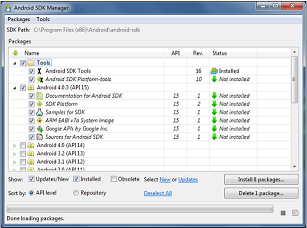
\includegraphics{Packages}
			\caption{Paquetes en SDK Manager}
			\label{fig:SdkManagerPackages}
		\end{figure}
		
	\newpage %Necesario para que la imagen aparezca antes de Firebase
	\subsection{Firebase}
		\begin{itemize}
			\item {\bf Librería}: Añadir la librería de Firebase en el archivo {\it ``build.gradle''} que esta dentro de la carpeta {\it ``app''} en el directorio raíz del proyecto.
				\lstinputlisting[float,language=Java,caption={Importación de la librería de {\it Firebase}},label={code:gradle}]{Code/build.gradle}
				
			\newpage
			\item {\bf Uso}: En los archivos de clase {\it ``java''}\cite{14:java:online} seguir los siguientes pasos:
				\begin{itemize}
					\item {\bf Librerías}: Se han de importar la librerías necesarias:
						\begin{itemize}
							\item {\bf Cliente Firebase}: Importar la librería del cliente.
							\item {\bf Errores Firebase}: Importar la librería de errores en consultas.
							\item {\bf Datos Firebase}: Importar la librería que permite la devolución de datos desde Firebase.
							\item {\bf Consultas Firebase}: Importar la librería para consultas.
							\item {\bf Librería Oyentes}: Importar la librería de los oyentes ({\it ``Listeners''}).
						\end{itemize}
					\item {\bf Contexto}: Añadir el contexto en que se va a usar en la función {\it onCreate}.
					\item {\bf Referencias}: Añadir una referencia a la base de datos o tabla de la misma a la que se van a hacer las consultas.
					\item {\bf Consultas}: Preparar la consulta que se va a hacer.
					\item {\bf Oyentes}: Añadir un oyente ({\it ``Listener''}) a la consulta.
				\end{itemize}
		\end{itemize}
		
		\lstinputlisting[float,language=Java,caption={Ejemplo de uso de {\it Firebase}},label={code:firebase}]{Code/FirebaseExample.java}
		
\newpage		
\section{Tutoriales}
	Antes de comenzar con el desarrollo de la aplicación, se han implementado varios tutoriales para afianzar los conocimientos sobre Android.
	\begin{enumerate}
		\item {\it Build your first app}\cite{29:firstapp:online} %En orden a partir de aquí
		\item {\it Adding the action bar}\cite{30:actionbar:online}
		\item {\it Supporting Different Devices}\cite{31:diferentdevices:online}
		\item {\it Managing the Activity Lifecycle}\cite{32:lifecycle:online}
		\item {\it Building a Dynamic UI with Fragments}\cite{33:fragments:online}
		\item {\it Saving Data}\cite{34:savingdata:online}
		\item {\it Interacting with Other Apps}\cite{35:interacting:online}
		\item {\it Sharing Simple Data}\cite{36:sharingsimpledata:online}
		\item {\it Sharing Files}\cite{37:sharingfiles:online}
		\item {\it Sharing Files with NFC}\cite{38:nfc:online}
		\item {\it Managing Audio Playback}\cite{39:audio:online}
		\item {\it Capturing Photos}\cite{40:photos:online}
		\item {\it Printing Content}\cite{41:printing:online}
		\item {\it Displaying Bitmaps Efficiently}\cite{42:bitmaps:online}
		\item {\it Displaying Graphics with OpenGL ES}\cite{43:opengl:online}
		\item {\it Animating Views Using Scenes and Transitions}\cite{44:transitions:online}
		\item {\it Adding Animations}\cite{45:animations:online}
		\item {\it Connecting Devices Wirelessly}\cite{46:connecting:online}
		\item {\it Performing Network Operations}\cite{47:networks:online}
		\item {\it Syncing to the Cloud}\cite{48:cloud:online}
		\item {\it Transferring Data Using Sync Adapters}\cite{49:adapters:online}
		\item {\it Best Practices for Security \& Privacy}\cite{50:securityprivacity:online}
		\item {\it Best Practices for Testing}\cite{51:testing:online}
		\item {\it Parse}\cite{52:parse:online}
		\item {\it Firebase Storage}\cite{53:firebase:online}
		\item {\it Expandable ListView}\cite{54:expandable:online}
		\item {\it TabHost Swipe}\cite{55:tabhostswipe:online}
		\item {\it ActionBar Tab Swipe}\cite{56:actionbartab:online}
	\end{enumerate} %A mandar
	%
% ---------------------------------------------------
%
% Trabajo de Final de Grado:
% Author: Gonzalo Jesús García Martín <dracoyue@gmail.com>
% Capítulo: Objetivos
% Fichero: Cap3_Objetivos.tex
%
% ----------------------------------------------------
%

\cleardoublepage
\chapter{Objetivos}
\label{chap:objetives}

	Se pretende crear una aplicación para dispositivos móviles, que utilicen como sistema operativo {\it Android} \cite{2:android:online}, como trabajo de fin de grado utilizando las nuevas tecnologías como los teléfonos inteligentes y los servicios de internet conocidos como Nube \cite{57:nube:online}. También se pretende adquirir las competencias relacionadas con la ingeniería del software y las ciencias de la computación. 
	
	A continuación se pasará a enumerar algunos de los objetivos específicos propuestos para este proyecto:
	
	\begin{itemize}
		\item Aplicar los conocimientos adquiridos en los estudios del Grado de Ingeniería Informática de la Universidad de La Laguna.
		\item Ampliar conocimientos sobre {\it Android}.
		\item Emprender el diseño y desarrollo de un proyecto.
		\item Adquirir conocimientos sobre el uso de servicios en la nube y su uso en aplicaciones {\it Android}.
		\item Gestión proyectos con {\it Github} \cite{9:github:online}: Plataforma de desarrollo colaborativo utilizada para el diseño y producción de software. Utiliza el {\it control de versiones git} \cite{5:git:online}.
		\item Crear una memoria técnica sobre la aplicación desarrollada en el presente Trabajo de Fin de Grado.
		\item Adquirir conocimientos sobre {\it Latex} \cite{8:latex:online}: Sistema de composición de textos, orientado a la creación de documentos escritos que presenten alta calidad tipográfica.
	\end{itemize} %A mandar
	%
% ---------------------------------------------------
%
% Trabajo de Final de Grado:
% Author: Gonzalo Jesús García Martín <dracoyue@gmail.com>
% Capítulo: Objetivos
% Fichero: Cap4_Antecedentes.tex
%
% ----------------------------------------------------
%

\cleardoublepage
\chapter{Antecedentes}
\label{chap:record}

	Con los nuevos avances tecnológicos se ha vuelto popular el uso de las comúnmente denominada {\it apps} en los dispositivos móviles. Hay aplicaciones para todos los gustos, desde lo más básico como aprender a cocinar o aplicaciones de comunicación, hasta de lo más importante como por ejemplo consultar la información de la cuenta del banco e incluso hacer operaciones con ella.
	
	\bigskip
	Se ha observado que en el ámbito docente hay una falta de comunicación entre padres y profesores. También el aumento de problemas como el acoso, fracaso escolar o incluso problemas de ámbito familiar influyen en los alumnos. Por eso los hasta ahora recursos tradicionales no eran suficientes. Notas escritas y reuniones no son más que informes puntuales de un progreso continuo que puede decaer sin aviso previo.
	
	\bigskip
	Por eso se presenta una herramienta que intenta establecer un flujo de información continua sin comprometer los datos personales de los usuarios tales como el teléfono o el correo. Así éstos se sentirán cómodos a la hora de comunicarse de forma segura. Se entiende que es un esfuerzo extra para los equipos docentes, pero permitirá que haya una mejor comunicación para resolver problemas inesperados y actuar de forma casi inmediata.
	
	\section{Otras Aplicaciones similares}
	
	A continuación se describirán aplicaciones similares a la que se ha desarrollado.
	
	\subsection{Remind}
	{\it Remind}\cite{3:remind:online} ofrece a los usuarios una forma sencilla de comunicación segura ya que los números de teléfono se mantienen confidenciales. Administradores o personal docente se pueden comunicar con los estudiantes y padres de forma personal, con un chat, o de forma generalizada enviando anuncios.
	
	\bigskip
	El profesor creará una o varias clases y obtendrá un código por cada clase que cree. Con este código los padres y alumnos podrán apuntarse a sus clases, recibiendo notificaciones o mensajes de los profesores, monitores y administradores. 
	
	En la figura \ref{fig:Remind} se puede apreciar la pantalla de bienvenida.
	
	\begin{figure}[h !]
		\centering
		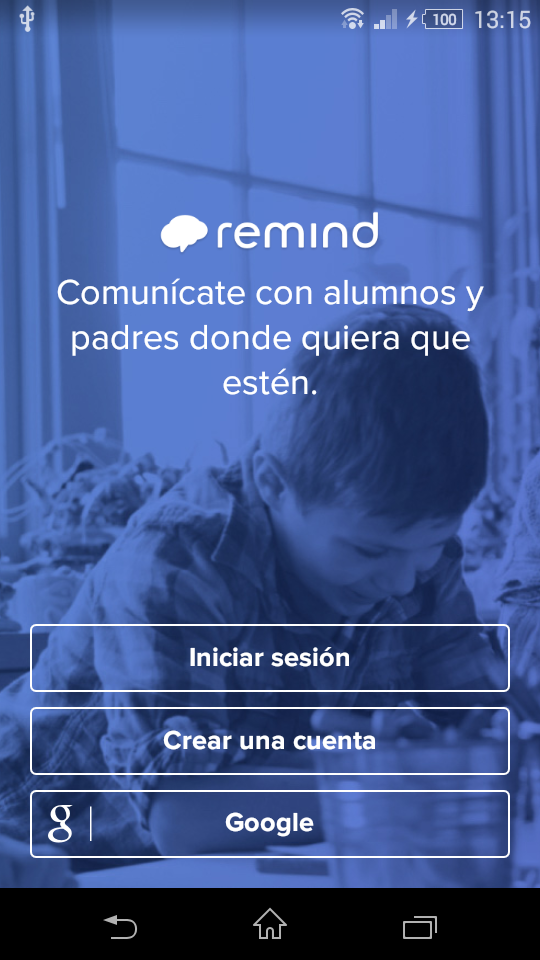
\includegraphics[scale=0.2]{Remind}
		\caption{Pantalla Bienvenida de la Aplicación Remind}
		\label{fig:Remind}
	\end{figure}
	
	\subsection{miColegioApp}
	En {\it miColegioApp}\cite{4:micolegioapp:online} el usuario se registra como alumno, profesor, padre, madre, tutor legal o persona autorizada. Una vez registrado, se solicita el código al centro, que debe haber contratado los servicios de la empresa previamente, y se introduce en la aplicación. Cuando se ha asociado al usuario con un centro, el dueño del dispositivo recibirá notificaciones y circulares del colegio.
	En la figura \ref{fig:miColegioApp} se observa la pantalla de inicio.
	
	\begin{figure}[h !]
		\centering
		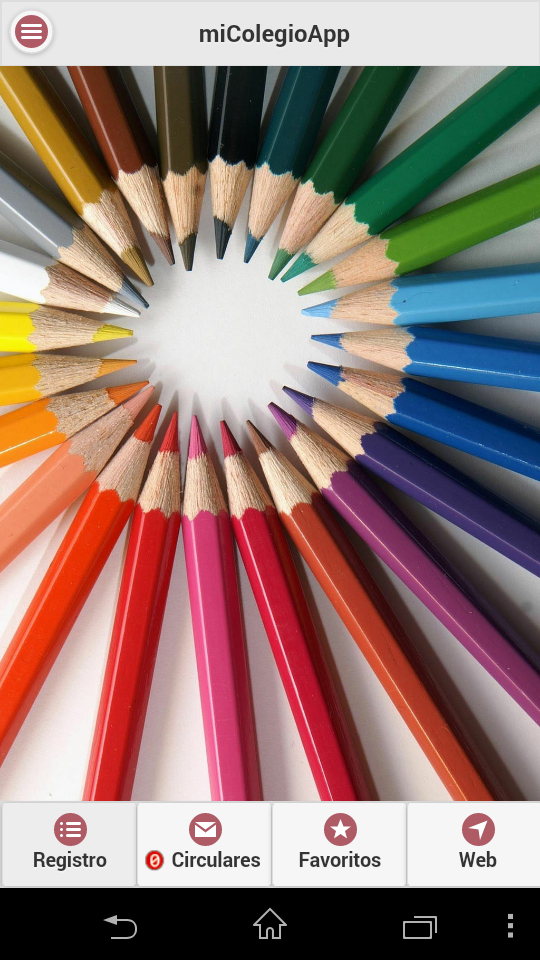
\includegraphics[scale=0.2]{miColegioApp}
		\caption{Pantalla Bienvenida de la Aplicación miColegioApp}
		\label{fig:miColegioApp}
	\end{figure} %A mandar
	%
% ---------------------------------------------------
%
% Trabajo de Final de Grado:
% Author: Gonzalo Jesús García Martín <dracoyue@gmail.com>
% Capítulo: Especificación de Requisitos
% Fichero: Cap2_EspecificacionRequisitos.tex
%
% ----------------------------------------------------
%

\cleardoublepage
\chapter{Especificación de Requisitos}
\label{chap:requirements}

	La especificación de requisitos es una parte fundamental de todo desarrollo ya que describe de forma completa el comportamiento funcional del software. Incluye casos de uso, requisitos funcionales, no funcionales, de usuarios y del sistema.
	Va dirigido tanto al cliente como al equipo de desarrollo y establece unos compromisos fundamentales entre ambos.
	
	\bigskip
	En este capítulo se describirán formalmente las funcionalidades, los sistemas integrados en la aplicación y los perfiles o roles que podrán tener los usuarios.
	
	\bigskip
	En el caso de \CollegeApp son varias las funcionalidades integradas en la aplicación, desde el registro y el acceso de usuarios hasta el envío de mensajes y la recepción notificaciones.
	
	\section{Funcionalidades}
		A continuación se describen las funcionalidades de la aplicación:
		\begin{itemize} 
			\item {\bf Registro}: Tras rellenar el formulario y accionar el botón de registro, \CollegeApp enviará los datos a un proveedor de servicios en la nube. Éstos serán almacenados en la base de datos, en sus tablas correspondientes. También creará al usuario para que tenga acceso a la aplicación.
			\item {\bf Acceso}: El usuario introducirá su dirección de correo electrónico y contraseña en los campos destinados a ello. El dispositivo móvil se autenticará contra el servidor y si todo es correcto permitirá el acceso.
			\item {\bf Recuerdo de Contraseña}: La aplicación solicitará al servicio en la nube una contraseña temporal para que el usuario pueda acceder, tras lo cual tendrá que editar su contraseña en \CollegeApp.
			\item {\bf Contactos}: Se recuperarán todos los usuarios relacionados con la persona que esté usando la aplicación. Esto permitirá que se puedan comunicar.
			\item {\bf Chat}: Los usuarios se podrán enviar mensajes entre sí, éstos se almacenaran en el servidor para ser recuperados por la aplicación y luego borrados de la nube. La comunicación será del tipo alumno-profesor, padre-profesor y viceversa en ambos casos. En ningún ámbito de la aplicación se permitirá la comunicación entre padres e hijos.
			\item {\bf Notificaciones}: \CollegeApp recuperará de la base de datos todos los mensajes que tenga el usuario, para después borrarlos de su almacenamiento en la nube. Éstas se diferenciarán por colores según el perfil del remitente.
			\item {\bf Circulares}: Aviso que enviará un profesor a todos los integrantes de una clase, e incluso de varias. Estos mensajes se almacenarán en la nube y serán recuperados por la aplicación, que los eliminará de su almacenamiento en internet.
			\item {\bf Citas}: Permitirá al usuario programar un evento en el calendario por defecto sin salir de la aplicación. Utiliza la funcionalidad para añadir eventos que implementa el sistema operativo\cite{5:os:online} del dispositivo. Se introducirán los datos en los campos correspondientes y se guardará la cita.
			\item {\bf Visualización de Datos}: El usuario podrá visualizar la información de sus contactos con una selección larga cualquiera de ellos.
			\item {\bf Modificación de datos}: El usuario podrá editar los datos en el dispositivo móvil, tras lo cual se actualizarán en la base de datos almacenada en la nube. 
			\item {\bf Darse de baja}: El usuario podrá eliminar su cuenta de la aplicación y su información en el servidor.
		\end{itemize}

	\section{Sistemas de la Aplicación}
		\begin{itemize}
			\item Sistema de Registro: Al usuario se le pedirán los siguientes datos:
			\begin{itemize}
				\item Nombre y Apellidos.
				\item Número de teléfono.
				\item D.N.I.
				\item Nombre del centro con el que va a hacer el registro.
				\item Clase y grupo.
				\item Correo electrónico y contraseña.
				\item En caso de que el usuario se registre como padre también tendrá que introducir:
				\begin{itemize}
					\item Nombre y Apellidos del alumno.
					\item D.N.I del alumno.
					\item Clase en la que está el alumno.
					\item Centro en el que está el alumno.
					\item Curso en el que está el alumno.
					\item Teléfono del alumno, este dato es opcional.
					\item Correo electrónico del alumno, este dato es opcional.
				\end{itemize}
			\end{itemize}
			\item Sistema de ``acceso'': Se le pedirá al usuario que ingrese su identificación, es decir, su correo electrónico y contraseña.
			\item Sistema de comunicación entre usuarios: Este servicio enviará los mensajes a través de internet usando los servicios de un proveedor. Se explicará en la siguiente tabla (Tabla \ref{table:communications}). %Pone tabla 4.2 cuando es la tabla 4.1
			
			\begin{table} [!hbt]
			\begin{center}
			\begin{tabular}{|| c | c | c | c ||}
				\hline
				\hline
				& Padre & Alumno & Profesor \\
				\hline
				Padre & Mensaje & Sin comunicación & Mensaje \\
				\hline
				Alumno & Sin comunicación & Mensaje & Mensaje \\
				\hline
				Profesor & Circular y Mensaje & Circular y Mensaje & Mensaje \\
				\hline
				\hline
			\end{tabular}
			\caption{Comunicaciones permitidas}
			\label{table:communications}
			\end{center}
			\end{table}
			
			No parece lógico que un usuario con el perfil de padre se pueda comunicar con los compañeros de clase de su hijo, puesto que no sería del agrado de los progenitores.
			\newline
			Las comunicaciones bidireccionales profesor-padre y profesor-alumno son necesarias para que los alumnos y los padres puedan recibir mensajes y notificaciones.
			
			\item Sistema de citas: Permitirá al usuario programar un evento en el calendario del dispositivo sin salir de la aplicación, usando las funciones que implementa Android.
			\item Lista de contactos: Organizada por grupos desplegables, por ejemplo los profesores tendrán la lista organizada según las clases que impartan en el centro.
		\end{itemize}
	
		Esto permitirá establecer un sistema de comunicaciones entre los profesores y padres de alumnos.

	\section{Perfiles}
		\begin{itemize}
			\item Alumnos: Podrán programar citas en el calendario y recibir circulares. Como se puede observar en la tabla \ref{table:studentsCommunications}, las comunicaciones entre alumnos y padres no están permitidas en ningún ámbito de la aplicación, ya que podría ocasionar problemas no deseados.
			Los estudiantes podrán conversar con los profesores para resolver las dudas y problemas que ellos consideren oportunos. También podrán comunicarse entre sí para pedir apuntes y resolver dudas entre otras cosas.
			
			\begin{table} [!hbt]
				\begin{center}
					\begin{tabular}{|| c | c | c | c ||}
						\hline
						\hline
						& Padre & Alumno & Profesor \\
						\hline
						Alumno & Sin comunicación & Mensaje & Mensaje \\
						\hline
						\hline
					\end{tabular}
					\caption{Comunicaciones permitidas para el perfil de alumno}
					\label{table:studentsCommunications}
				\end{center}
			\end{table}
			
			\item Profesores: Podrán programar citas en el calendario y enviar circulares. Los padres y alumnos en la lista de contactos estarán organizados según las clases que impartan en el centro. Como se explica en la tabla \ref{table:teachersCommunications}, los profesores se pueden comunicar con todos los usuarios a través de mensajes directos tipo chat, mientras que con los padres y alumnos, además, pueden usar mensajes tipo circulares que le llegarán a todos los integrantes de la clase. Esto cumple con el objetivo de que tanto alumnos como padres estén informados de las incidencias ocurridas en clase.
			
			\begin{table} [!hbt]
				\begin{center}
					\begin{tabular}{|| c | c | c | c ||}
						\hline
						\hline
						& Padre & Alumno & Profesor \\
						\hline
						Profesor & Circular y Mensaje & Circular y Mensaje & Mensaje \\
						\hline
						\hline
					\end{tabular}
					\caption{Comunicaciones permitidas para el perfil de profesor.}
					\label{table:teachersCommunications}
				\end{center}
			\end{table}
			
			\item Padre/Madre/Tutor Legal: Podrán recibir circulares y programar citas en el calendario. Los profesores y padres en la lista de contactos estarán organizados según las clases que impartan a los alumnos con los que el progenitor esté relacionado.
			En la tabla \ref{table:fathersCommunications} se puede observar que los padres se pueden comunicar con los profesores para estar informados de todo lo que ocurre con sus hijos.
			
			\begin{table} [!hbt]
				\begin{center}
					\begin{tabular}{|| c | c | c | c ||}
						\hline
						\hline
						& Padre & Alumno & Profesor \\
						\hline
						Padre & Mensaje & Sin comunicación & Mensaje \\
						\hline
						\hline
					\end{tabular}
					\caption{Comunicaciones permitidas para el perfil de padre.}
					\label{table:fathersCommunications}
				\end{center}
			\end{table}
			
			
		\end{itemize}
 %A mandar
	%
% ---------------------------------------------------
%
% Trabajo de Final de Grado:
% Author: Gonzalo Jesús García Martín <dracoyue@gmail.com>
% Capítulo: Introducción
% Fichero: Cap4_Herramientas.tex
%
% ----------------------------------------------------
%

\cleardoublepage
\chapter{Herramientas}
\label{chap:tools}

	El software usado en el desarrollo de \CollegeApp\ ha sido el siguiente:
	\begin{itemize}
		\item {\bf AndroidStudio} \cite{1:androidstudio:online}: Entorno de desarrollo integrado oficial para el desarrollo de aplicaciones para {\it Android}, basado en {\it IntelliJ IDEA} \cite{14:intellij:online}.
		Ha sido seleccionado por ser un entorno de programación moderno, de uso intuitivo y ligero en comparación con otros entornos de desarrollo ya existentes como {\it eclipse} \cite{15:eclipse:online} o {\it netbeans} \cite{22:netbeans:online} que son más pesados, ya que soportan más lenguajes de programación.
		\item {\bf Android} \cite{2:android:online}: Sistema operativo basado en el {\it núcleo de Linux} para dispositivos móviles, televisores, automóviles y relojes inteligentes.
		\item {\bf Firebase} \cite{6:firebase:online}: Proveedor de contenidos que proporciona servicios en la nube de forma fácil y segura, con una integración sencilla con las nuevas tecnologías. Ofrece servicios de recuperación y almacenamiento de datos, registro y acceso de usuarios, reglas de seguridad, simulador y análisis de datos entre otros. Los datos almacenados en este servicio no son datos \href{http://es.wikipedia.org/wiki/SQL}{\textit{SQL}}, sino que son datos \href{http://es.wikipedia.org/wiki/JSON}{\textit{JSON}} \cite{7:json:online}. Ha sido elegido por ser uno de los servicios en la nube más sencillos de utilizar.
		Sistemas con los que {\it Firebase} está integrado:
		\begin{itemize}
			\item {\bf Android}: Sistema Operativo para dispositivos móviles propiedad de Google.
			\item {\bf IOS} \cite{16:ios:online}: Sistema operativo para dispositivos móviles propiedad de Apple Inc.
			\item {\bf Servicios Web}.
			\item {\bf Servicios REST} \cite{18:rest:online}: Es un conjunto de principios de arquitectura, pero en la actualidad se usa en el sentido más amplio para describir cualquier interfaz entre sistemas que utilice directamente HTTP \cite{60:http:online} para obtener datos o indicar la ejecución de operaciones sobre los datos, en cualquier formato sin las abstracciones adicionales de los protocolos basados en patrones de intercambio de mensajes, como por ejemplo SOAP \cite{56:soap:online}.
		\end{itemize}
	\end{itemize}
	
	\section{Otros Servicios en la Nube: Parse \cite{16:parse:online}}
	Proveedor de servicios en la nube alternativo a {\it Firebase} que ofrece eventos, autenticación de usuarios, almacenamientos de datos, análisis y {\it notificaciones push} entre otros.
	
	\bigskip
	Tras la implementación de una aplicación ejemplo para valorar {\it Parse}, se ha seleccionado {\it Firebase} por estar diseñado para la construcción de datos en tiempo real. Al acceder a través de una librería cliente los datos se sincronizan en tiempo real rápidamente. También ofrece una {\it interfaz de programación de aplicaciones} \cite{23:api:online}  de seguridad basada en la expresión altamente flexible que permite un control preciso sobre el acceso a los datos de los clientes.
	
	\bigskip
	{\it Parse} está integrado con las siguientes tecnologías:
	\begin{itemize}
		\setlength{\itemsep}{1pt}
		\setlength{\parskip}{0pt}
		\setlength{\parsep}{0pt}
		\item {\it IOS}.
		\item {\it Android} \cite{2:android:online}.
		\item {\it Javascript}.
		\item {\it OSX}.
		\item {\it Unity}: Software para la creación de videojuegos.
		\item {\it PHP}: Lenguaje de programación.
		\item {\it .Net + Xamarin}.
		\item {\it Arduino}: Hardware libre que consiste en una placa con un microcontrolador y un entorno de programación.
		\item {\it Embedded C}: Lenguaje de programción que extiende sus funcionalidades de C.
		\item {\it Servicios REST}.
	\end{itemize}
	
	\subsubsection{Instalación}
	\begin{itemize}
		\item {\bf Descarga}: Descargar librería de {\it Parse}.
		\item {\bf Librería}: Añadir la librería de {\it Parse} en el archivo {\ttfamily build.gradle} que esta dentro de la carpeta {\ttfamily app} en el directorio raíz del proyecto. Véase listado \ref{code:gradleParse}

		\lstinputlisting[float = h!,language=Java,caption={Importación de la librería de {\it Parse}},label={code:gradleParse}]{Code/buildParse.gradle}
		\newpage
		
		\item {\bf Uso}: En los archivos de clase {\ttfamily  .java}\ \cite{19:java:online} seguir los siguientes pasos:
		\begin{itemize}
			\item {\bf Librerías}: Importar las librerías necesarias:
			\begin{itemize}
				\item {\bf Cliente Firebase}: Importar la librería del cliente.
				\item {\bf Consultas}: Importar la librería de consultas ({\ttfamily ParseQuery}).
				\item {\bf Listeners}: Importar la librería de oyentes ({\ttfamily FindCallback}).
				\item {\bf Excepciones}: Importar la librería de excepciones ({\ttfamily ParseException}).
				\item {\bf Objetos}: Importar la librería de objetos ({\ttfamily ParseObject}).
				\item {\bf Usuarios}: Importar la librería de atenticación de usuarios ({\ttfamily ParseUser}).
			\end{itemize}
			\item {\bf Claves}: Crear dos contantes de tipo cadena ({\it String}) en las introduciremos manualmente la identificación de la aplicación ({\it AppID}) y la clave del cliente ({\it CLIENT\_KEY}).
			\item {\bf Contexto}: Añadir el contexto en que se va a usar en la función {\ttfamily onCreate()} con la identificación y la clave.
			\item {\bf Consultas}: Preparar la consulta que se va a hacer.
			\item {\bf Oyentes}:Añadir un oyente ({\it Listener}) a la consulta.
		\end{itemize}
		
		En el listado \ref{code:parse} se presenta un ejemplo de uso de la librería.
		
		\newpage
		\noindent
		\lstinputlisting[language=Java,caption={Ejemplo de uso de {\it Parse} (parte del código)},label={code:parse}]{Code/ParseExample.java}
	\end{itemize}
		
	\section{Instalación de las herramientas usadas}
	En esta sección se procederá a explicar la instalación de {\it AndroidStudio} y {\it Firebase}.
	
	\subsection{AndroidStudio}
	\begin{itemize}
		\item {\bf JDK}: Descargar e instalar {\it Java Development Kit} \cite{17:jdk:online}.
		\item {\bf Descarga}: Descargar {\it AndrodiStudio}.
		\item {\bf Instalación}: Ejecutar el archivo de instalación descargado y seguir los pasos indicados por el instalador.
		\item {\bf SDK}: Añadir paquetes {\it SDK} con el gestor de paquetes ({\it SDK Manager}) seleccionándolo en la barra de herramientas.
		\item {\bf Paquetes}: Seleccionar las versiones de {\it Android} \cite{2:android:online} a instalar, se pueden elegir o quitar paquetes concretos de cada versión. Darle a {\it Install}. Es importante que ademas de instalar las versiones a utilizar, se instalen los siguientes paquetes:
		\begin{itemize}
			\item {\it Android SDK Tools}.
			\item {\it Android SDK Platform-tools}.
			\item {\it Android SDK Build-tools} (La versión más actual).
			\item Extras \textgreater {\it Android Support Repository}.
			\item Extras \textgreater {\it Android Support Library}.
			\item Extras \textgreater {\it Google USB Driver}.
		\end{itemize}
	\end{itemize}
	
	En la figura \ref{fig:SdkManagerPackages} se pueden observar los paquetes que se pueden instalar.
	
	\begin{figure}[h !]
		\centering
		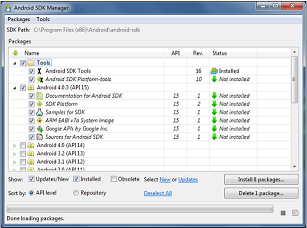
\includegraphics[scale=0.5]{Packages}
		\caption{Paquetes en SDK Manager}
		\label{fig:SdkManagerPackages}
	\end{figure}
	
	\newpage
	\subsection{Firebase}
	\begin{itemize}
		\item {\bf Librería}: Añadir la librería de {\it Firebase} en el archivo {\ttfamily build.gradle} que está dentro de la carpeta {\ttfamily app} en el directorio raíz del proyecto \CollegeApp. En el listado \ref{code:gradle} se puede observar cómo se importa la librería de {\it Firebase}.
		
		\lstinputlisting[float = h!,language=Java,caption={Importación de la librería de {\it Firebase}},label={code:gradle}]{Code/build.gradle}
		
		\item {\bf Uso}: En los archivos de clase {\ttfamily .java }\cite{19:java:online} seguir los siguientes pasos:
		\begin{itemize}
			\item {\bf Librerías}: Se han de importar la librerías necesarias:
			\begin{itemize}
				\item {\bf Cliente Firebase}: Importar la librería del cliente.
				\item {\bf Errores Firebase}: Importar la librería de errores en consultas.
				\item {\bf Datos Firebase}: Importar la librería que permite la devolución de datos desde {\it Firebase}.
				\item {\bf Consultas Firebase}: Importar la librería para consultas.
				\item {\bf Librería Oyentes}: Importar la librería de los oyentes ({\it Listeners}).
			\end{itemize}
			\item {\bf Contexto}: Añadir el contexto en que se va a usar en la función {\ttfamily onCreate()}.
			\item {\bf Referencias}: Añadir una referencia a la base de datos o tabla de la misma a la que se van a hacer las consultas.
			\item {\bf Consultas}: Preparar la consulta que se va a hacer.
			\item {\bf Oyentes}: Añadir un oyente ({\it Listener}) a la consulta.
		\end{itemize}
	\end{itemize}

	En el listado \ref{code:firebase} se presenta un ejemplo del uso de la librería {\it Firebase}.
	
	\lstinputlisting[float = h!,language=Java,caption={Ejemplo de uso de {\it Firebase}},label={code:firebase}]{Code/FirebaseExample.java}
	
	\section{Tutoriales}
	
	Antes de comenzar con el desarrollo de la aplicación propiamente dicha, se han implementado diversas aplicaciones a modo de ejemplo para afianzar los conocimientos sobre {\it Android}.
	
	\begin{enumerate}
		\setlength{\itemsep}{1pt}
		\setlength{\parskip}{0pt}
		\setlength{\parsep}{0pt}
		\item {\it Build your first app} \cite{29:firstapp:online}
		\item {\it Adding the action bar}
		\item {\it Supporting Different Devices} \label{tut:3}
		\item {\it Managing the Activity Lifecycle}
		\item {\it Building a Dynamic UI with Fragments} \label{tut:5}
		\item {\it Saving Data}
		\item {\it Interacting with Other Apps}
		\item {\it Sharing Simple Data}
		\item {\it Sharing Files}
		\item {\it Sharing Files with NFC}
		\item {\it Managing Audio Playback}
		\item {\it Capturing Photos}
		\item {\it Printing Content}
		\item {\it Displaying Bitmaps Efficiently}
		\item {\it Displaying Graphics with OpenGL ES}
		\item {\it Animating Views Using Scenes and Transitions}
		\item {\it Adding Animations} \label{tut:17}
		\item {\it Connecting Devices Wirelessly}
		\item {\it Performing Network Operations}
		\item {\it Syncing to the Cloud}
		\item {\it Transferring Data Using Sync Adapters}
		\item {\it Best Practices for Security \& Privacy}
		\item {\it Best Practices for Testing}
		\item {\it Parse}
		\item {\it Firebase Storage} \label{tut:25}
		\item {\it Expandable ListView} \label{tut:26}
		\item {\it TabHost Swipe} \cite{55:tabhostswipe:online} \label{tut:27}
		\item {\it ActionBar Tab Swipe} \label{tut:28}
	\end{enumerate}
	
	Los tutoriales más relevantes para el desarrollo de \CollegeApp\ fueron {\it Supporting Different Devices} (tutorial \ref{tut:3}) que ayudó a implementar el soporte de idiomas y {\it Building a Dynamic UI with Fragments} (tutorial \ref{tut:5}), {\it ActionBar Tab Swipe} (tutorial \ref{tut:28}) y {\it TabHost Swipe} (tutorial \ref{tut:27}) gracias a los cuales existe {\ttfamily WelcomeActivity}.
	
	 También han sido significativos {\it Adding Animations} (tutorial \ref{tut:17}) para el {\it cuadro de diálogo} {\bf cargando}, {\it Firebase Storage} (tutorial \ref{tut:25}) que permitió la programación del uso de la base de datos y {\it Expandable ListView} (tutorial \ref{tut:26}) cuyos conocimientos se utilizaron en el desarrollo de la lista de contactos desplegable. %A mandar
	%
% ---------------------------------------------------
%
% Trabajo de Final de Grado:
% Author: Gonzalo Jesús García Martín <dracoyue@gmail.com>
% Capítulo: Introducción
% Fichero: Cap6_DescripcionApp.tex
%
% ----------------------------------------------------
%

\cleardoublepage
\chapter{Descripción de la Aplicación}
\label{chap:description}

	En este capítulo se hará una descripción de la interfaz gráfica y de cada una de las funcionalidades de las pantallas de \CollegeApp. Antes de comenzar con este apartado debemos explicar unos términos:
	
	\begin{itemize}
		\item {\it Activity}: Componente del modelo Vista-Controlador usado por Android y que provee al usuario de una interfaz gráfica. También llamado actividad.
		\item {\it Fragment}: Representa un comportamiento o un elemento de interfaz de usuario en una actividad. Puede combinar varios fragmentos en una sola actividad para construir una interfaz de usuario con varios paneles y reutilizar un fragmento en múltiples actividades. También conocido como fragmento.
		\item {\it Dialog}: Es una pequeña ventana que pide al usuario que tomar una decisión o introducir información adicional. No ocupa toda la pantalla y se utiliza normalmente para eventos modales que requieren que los usuarios tomen una acción antes de que puedan proceder. También conocido como cuadro de diálogo.
	\end{itemize}
	
	\section{Pantalla Principal (MainActivity)}
		La pantalla principal es a la que accede el usuario cuando inicia la aplicación. Esta se compone de tres {\it fragments}.
		
		\subsection{Bienvenida (WelcomeFragment)} \label{sec:welcome}
			El pantalla que le da la bienvenida al usuario. Como se puede ver en la figura \ref{fig:welcome}, contiene dos botones. Un botón que lleva a la pantalla de registro (ver sección \ref{sec:register}) y otro que lleva a la pantalla de acceso a la aplicación (ver sección \ref{sec:login}).
			
			\begin{figure}[h !]
				\centering
				
\includegraphics[scale=0.2]{Imagenes/App/welcome}
				\caption{Pantalla de Bienvenida de la Aplicación.}
				\label{fig:welcome}
			\end{figure}
		
		\subsection{Ayuda (HelpFragment)}
			
			En la figura \ref{fig:help} se puede observar una ayuda orientada al uso de la aplicación. Los usuarios pueden consultar en esta pantalla todo lo referente a \CollegeApp. El usuario puede deslizar la pantalla para ver toda la información.
			
			\begin{figure}[h !]
				\centering
				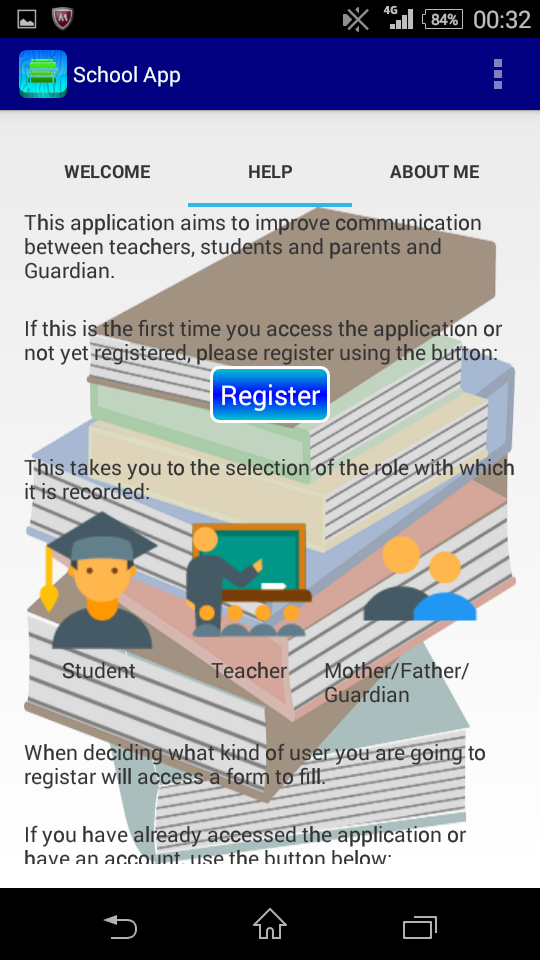
\includegraphics[scale=0.2]{Imagenes/App/help}
				\caption{Pantalla de ayuda de la Aplicación.}
				\label{fig:help}
			\end{figure}
		
		\subsection{Sobre mi (AboutMeFragment)}
			En la figura \ref{fig:aboutMe} se puede observar información referente al autor de la aplicación.
		
			\begin{figure}[h !]
				\centering
				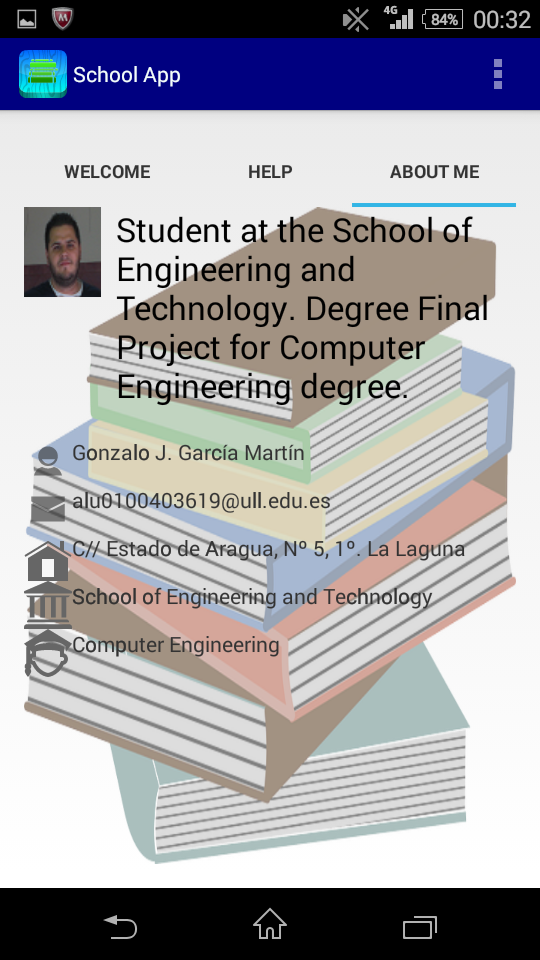
\includegraphics[scale=0.2]{Imagenes/App/aboutMe}
				\caption{Pantalla sobre el autor de la Aplicación.}
				\label{fig:aboutMe}
			\end{figure}
	
	\section{Cambio de idioma (ChangeLanguajeActivity)}
	
		En la figura \ref{fig:languaje} se puede observar los distintos idiomas disponibles de la aplicación. Al seleccionar uno de ellos y accionar el botón volver, quedará almacenado el idioma y las actividades lo cargarán al ser creadas.
	
		\begin{figure}[h !]
			\centering
			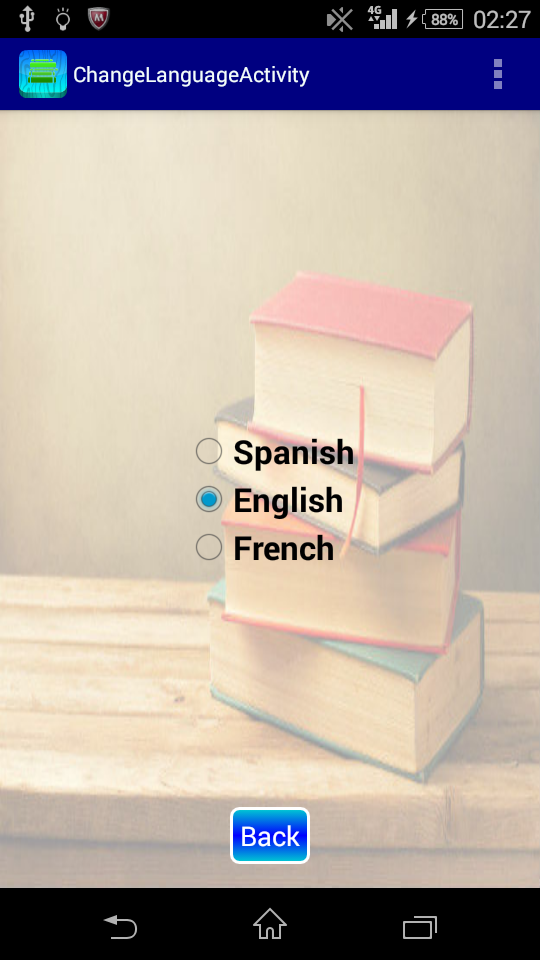
\includegraphics[scale=0.2]{Imagenes/App/ChangeLanguaje}
			\caption{Pantalla de cambio de idioma.}
			\label{fig:languaje}
		\end{figure}
			
	\section{Registro (RegisterActivity)} \label{sec:register}
		
		En la pantalla de registro (figura \ref{fig:register}) se pueden observar los perfiles con los que se puede registrar un usuario. Al seleccionar cualquiera de los tres botones, mostrará la pantalla de registro correspondiente.
		
		\begin{figure}[h !]
			\centering
			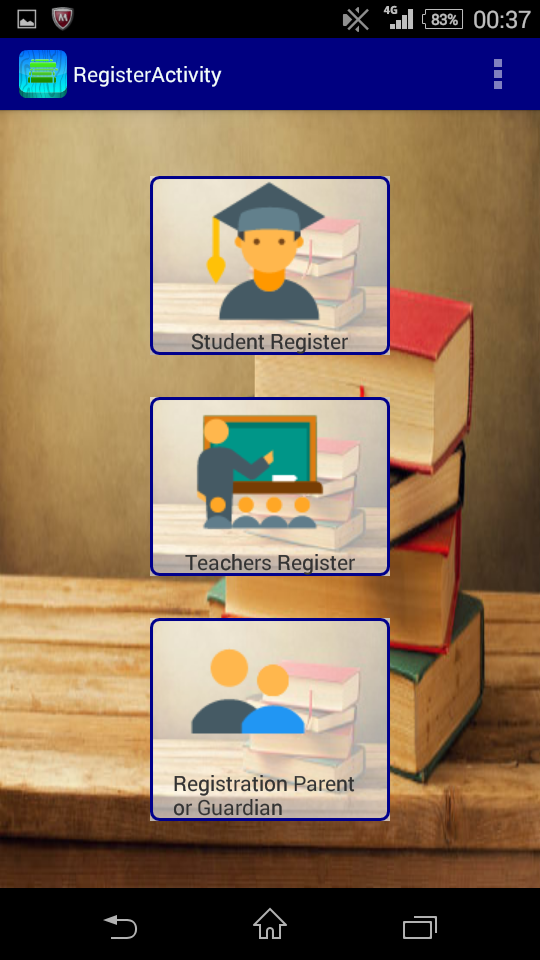
\includegraphics[scale=0.2]{Imagenes/App/registro}
			\caption{Pantalla de selección de perfil para el registro.}
			\label{fig:register}
		\end{figure}
		
		
		\subsection{Registro de alumnos (RegisterStudentActivity)} \label{sec:StudentRegister}
			
			La pantalla de registro de alumnos (figura \ref{fig:StudentRegister}) presenta un formulario que el usuario deberá rellenar. Presenta dos botones, uno que le devolverá a la pantalla de bienvenida (sección \ref{sec:welcome}) y otro que completará el registro. La aplicación solo permitirá el registro si se han rellenado todos los campos obligatorios. Una vez hecho, al accionar el botón, la aplicación llevará a cabo el registro del usuario en la base de datos de {\it Firebase}. También se accederá de forma automática a la aplicación.
			
			\begin{figure}[h !]
				\centering
				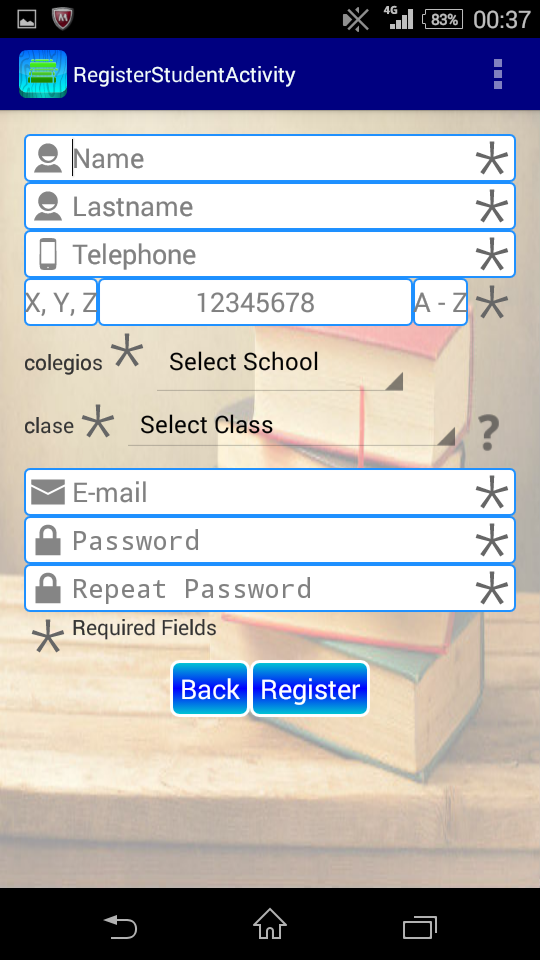
\includegraphics[scale=0.2]{Imagenes/App/registroAlumno}
				\caption{Registro de alumnos.}
				\label{fig:StudentRegister}
			\end{figure}
			
		\subsection{Registro de Profesores (RegisterTeacherActivity)}
		
			La pantalla de registro de profesor funciona exactamente igual que la pantalla de registro de alumno. Véase sección \ref{sec:StudentRegister}.
		
			\begin{figure}[h !]
				\centering
				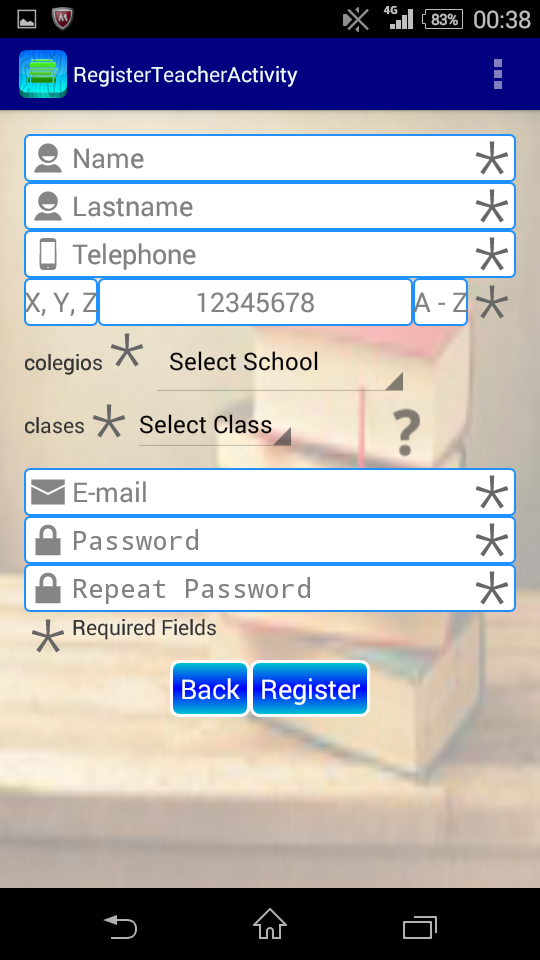
\includegraphics[scale=0.2]{Imagenes/App/registroProfe}
				\caption{Registro de profesores.}
				\label{fig:teacherRegister}
			\end{figure}
		
		\subsection{Registro de Padres (RegisterFatherActivity)} \label{sec:FatherRegister}
		
			La pantalla de registro de padre (figura \ref{fig:fatherRegister}) funciona exactamente igual que la de registro de alumnos, con la salvedad de que al usar el perfil de padre se debe al menos registrar un hijo para que el registro se lleve a cabo. Para llevar a cabo el registro de un hijo acciónese el botón con el símbolo de suma. Véase sección \ref{sec:addChild}.
			
			\begin{figure}[h !]
				\centering
				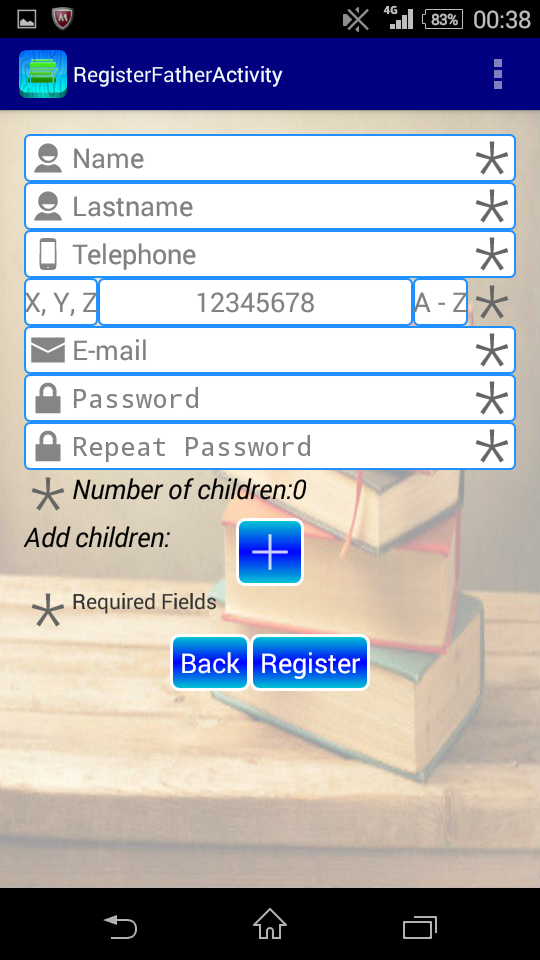
\includegraphics[scale=0.2]{Imagenes/App/registroPadre}
				\caption{Registro de padres.}
				\label{fig:fatherRegister}
			\end{figure}
			
		\subsection{Añadir hijo (AddChildActivity)} \label{sec:addChild}
			
			A esta pantalla (figura \ref{fig:addChildRegister}) se accede desde la pantalla de registro de padres (sección \ref{sec:FatherRegister}). Al introducir los datos del estudiante (sección \ref{sec:StudentRegister}), la aplicación consultará a la base de datos si existe el alumno. Si no existe se añadirá la información y se asociará con el padre, mientras que si existe solo se asociará. Tras el registro del alumno volverá a mostrar la pantalla de registro de padres (sección \ref{sec:FatherRegister}).
			
			\begin{figure}[h !]
				\centering
				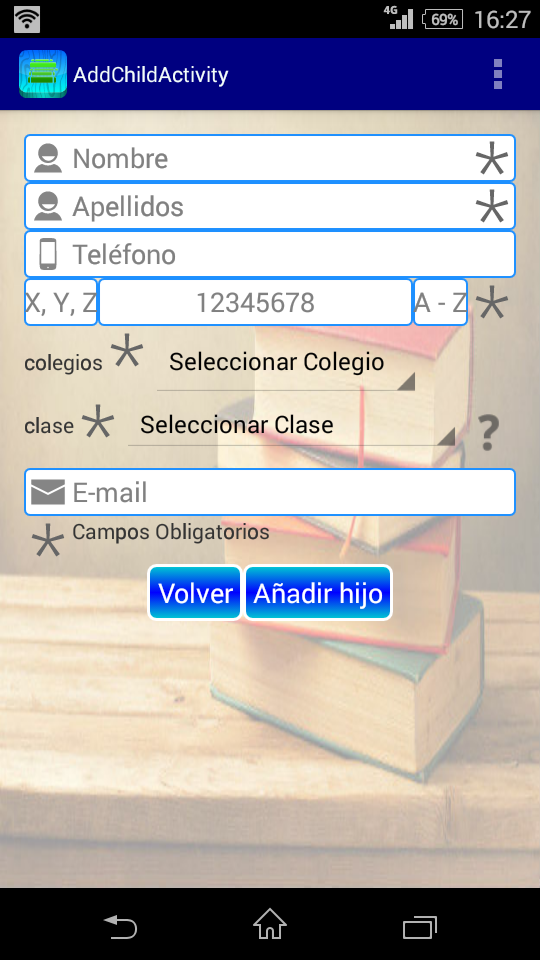
\includegraphics[scale=0.2]{Imagenes/App/addChild}
				\caption{Registro de hijos.}
				\label{fig:addChildRegister}
			\end{figure}
		
	\section{Acceso (LoginActivity)} \label{sec:login}
		
		En la pantalla de acceso (figura \ref{fig:login}) se puede observar que el usuario debe introducir su correo electrónico y contraseña para poder acceder a \CollegeApp con el botón de acceso. Si selecciona el de registro, se mostrará la pantalla de selección de perfil (Véase \ref{sec:register}). Para seleccionar {\it nueva contraseña} el usuario debe haber introducido previamente su correo electrónico. La aplicación se la solicitará al servidor de {\it Firebase} quien la mandará a la dirección con la que el usuario se ha registrado.  
		
		\begin{figure}[h !]
			\centering
			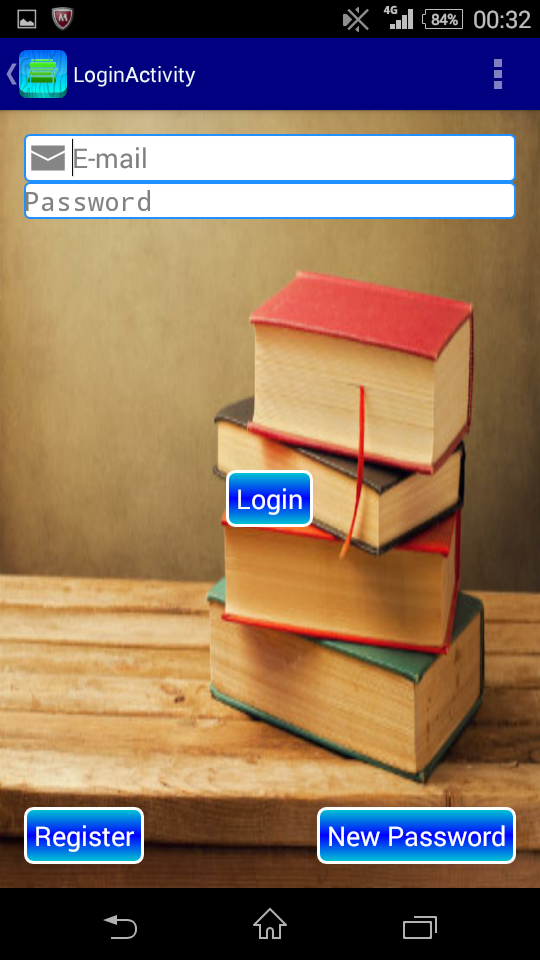
\includegraphics[scale=0.2]{Imagenes/App/login}
			\caption{Pantalla de acceso.}
			\label{fig:login}
		\end{figure}
		
		\bigskip
		En la figura \ref{fig:loginLand} se puede observar la pantalla de acceso con el dispositivo en horizontal.
		
		\begin{figure}[h !]
			\centering
			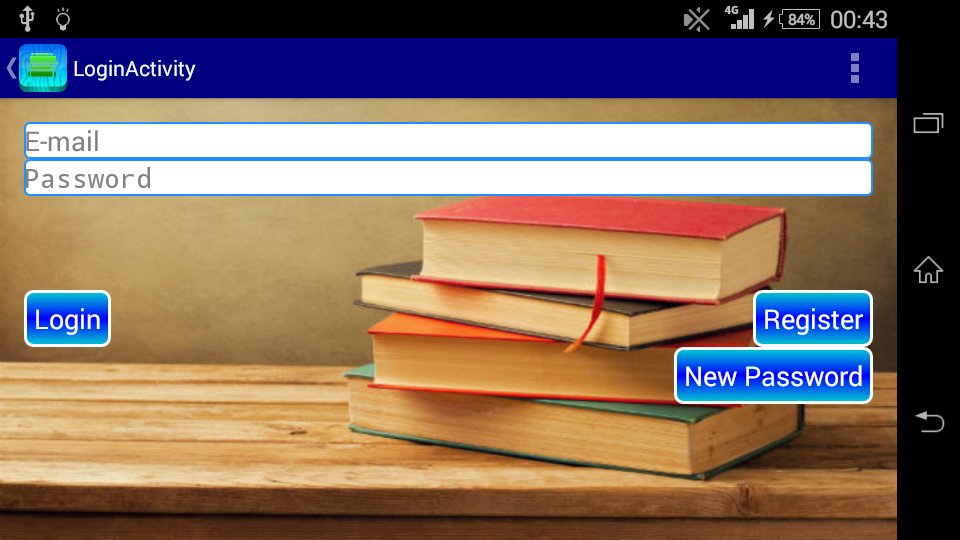
\includegraphics[scale=0.2]{Imagenes/App/loginLand}
			\caption{Pantalla de acceso con el dispositivo en horizontal.}
			\label{fig:loginLand}
		\end{figure}
		
	\section{Acceso como alumno (StudentTabActivity)}
		
		En esta pantalla se mostrarán en pestañas las listas de contactos de los usuarios con el perfil de alumno. También se mostrará una pestaña adicional para las notificaciones, es decir, mensajes que le lleguen al alumno (sección: \ref{sec:notifications}). En las opciones puede seleccionar cambiar sus datos (sección \ref{sec:myData}) y salir de la aplicación.
		Al seleccionar el botón citas (sección \ref{sec:dates}) se mostrará la pantalla encargada de añadir un evento al calendario del dispositivo. Esta funcionalidad viene implementada por el {\it sistema operativo}.
		
		\subsection{Lista de contactos: Alumnos (studentActivity)}
			
			En la figura \ref{fig:aluAlu} se puede observar los contactos que son compañeros de clase del alumno. Al seleccionar cualquiera de los contactos se podrá comunicar de forma directa con mensajes tipo chat (sección \ref{sec:chat}). Al hacer una selección larga podrá ver la información del contacto (sección \ref{sec:data}).
			
			\begin{figure}[h !]
				\centering
				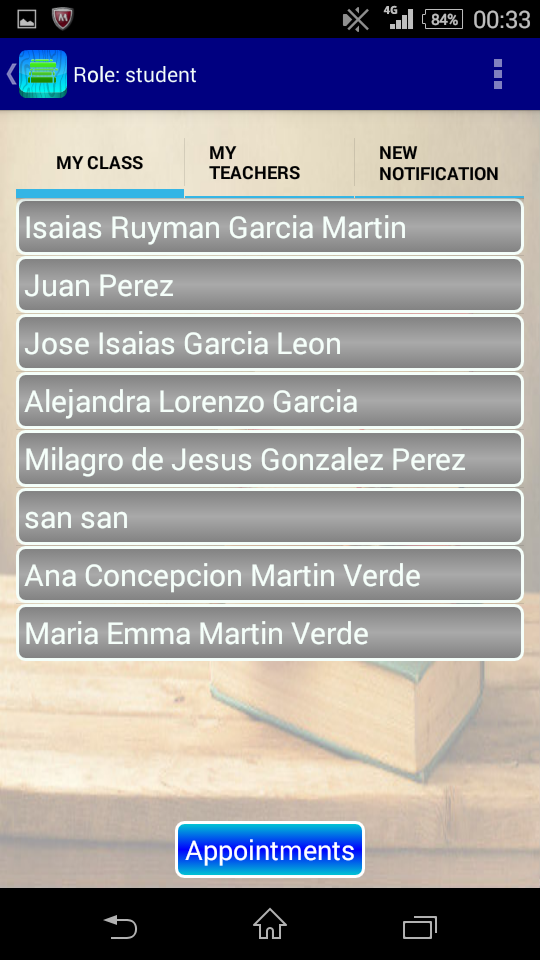
\includegraphics[scale=0.2]{Imagenes/App/aluAlu}
				\caption{Lista de contacto de alumnos para el perfil de alumno.}
				\label{fig:aluAlu}
			\end{figure}
			
		\subsection{Lista de contactos: Profesores (TeachersActivity)}
		
			En esta pantalla (figura \ref{fig:aluProfe}) se pueden ver los contactos que son profesores y le dan clase al usuario. Al seleccionar cualquiera de los contactos se podrá comunicar de forma directa con mensajes tipo chat (sección \ref{sec:chat}). Al hacer una selección larga podrá ver la información del contacto (sección \ref{sec:data}).
		
			\begin{figure}[h !]
				\centering
				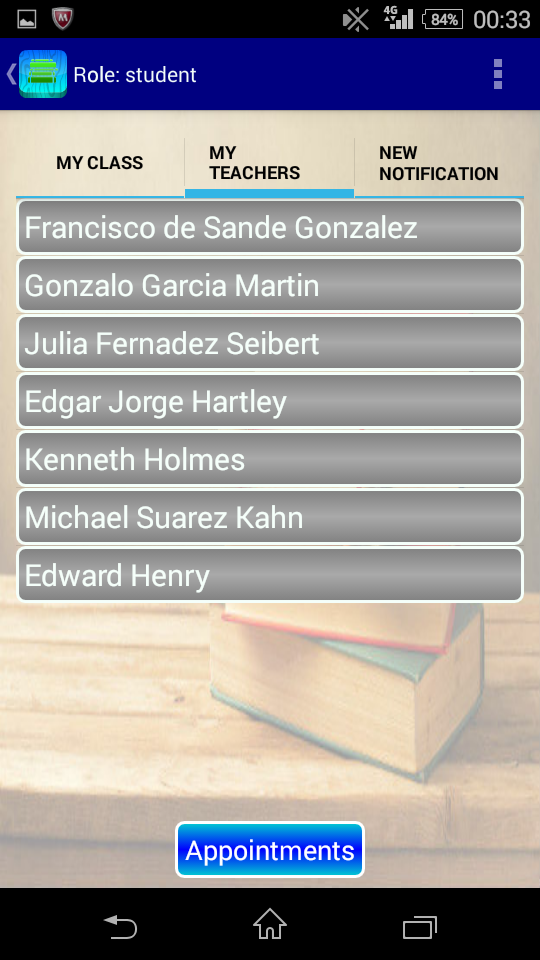
\includegraphics[scale=0.2]{Imagenes/App/aluProfe}
				\caption{Lista de contacto de profesores para el perfil de alumno.}
				\label{fig:aluProfe}
			\end{figure}
		
	\section{Acceso como padre (FatherTabActivity)}
	
		En esta pantalla se mostrarán en pestañas las listas de contactos de los usuarios con el perfil de padre. También se mostrará una pestaña adicional para las notificaciones, es decir, mensajes que le lleguen al padre (sección: \ref{sec:notifications}). En las opciones puede seleccionar cambiar sus datos (sección \ref{sec:myData}) y salir de la aplicación.
		Al seleccionar el botón citas (sección \ref{sec:dates}) se mostrará la pantalla encargada de añadir un evento al calendario del dispositivo. Esta funcionalidad viene implementada por el {\it sistema operativo}.
		
		\subsection{Lista de contactos: Padres (ExpandableFathersActivity)}
		
			En la figura \ref{fig:padrePadre} se puede observar la lista de contactos de padres para los usuarios con el mismo perfil. Estarán organizados según las clases en las que tengan algún hijo. Al seleccionar cualquier contacto se podrá comunicar de forma directa con mensajes tipo chat (sección \ref{sec:chat}). Al hacer una selección larga podrá ver la información del contacto (sección \ref{sec:data}).
			
			\begin{figure}[h !]
				\centering
				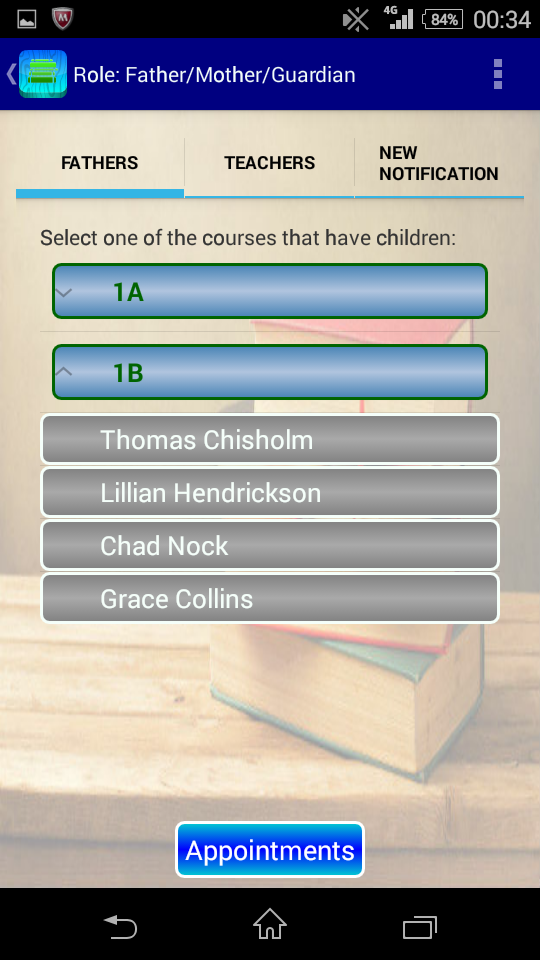
\includegraphics[scale=0.2]{Imagenes/App/padrePadre}
				\caption{Lista de contacto de padres para el perfil de padre.}
				\label{fig:padrePadre}
			\end{figure}
		
		\subsection{Lista de contactos: Profesores (ExpandableTeachersActivity)}
		
			En esta pantalla (figura \ref{fig:padreProfe}) se puede observar la lista de contactos de profesores para los usuarios con el perfil de padre. Estarán organizados según los profesores que den clases en las clases en las que tengan algún hijo. Al seleccionar cualquiera de los contactos se podrá comunicar de forma directa con mensajes tipo chat (sección \ref{sec:chat}). Al hacer una selección larga podrá ver la información del contacto (sección \ref{sec:data}).
		
			\begin{figure}[h !]
				\centering
				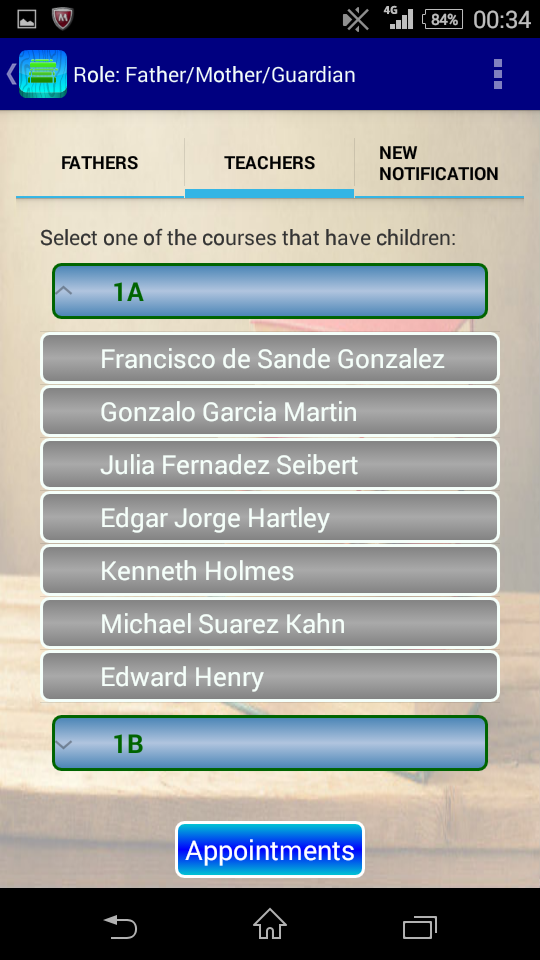
\includegraphics[scale=0.2]{Imagenes/App/padreProfe}
				\caption{Lista de contacto de profesores para el perfil de padre.}
				\label{fig:padreProfe}
			\end{figure}
		
	\section{Acceso como profesor (TeacherTabActivity)}
	
		En esta pantalla se mostrarán en pestañas las listas de contactos de los usuarios con el perfil de profesor. También se mostrará una pestaña adicional para las notificaciones, es decir, mensajes que le lleguen al padre (sección: \ref{sec:notifications}). En las opciones puede seleccionar cambiar sus datos (sección \ref{sec:myData}) y salir de la aplicación.
		Al seleccionar el botón citas (sección \ref{sec:dates}) se mostrará la pantalla encargada de añadir un evento al calendario del dispositivo. Esta funcionalidad viene implementada por el {\it sistema operativo}. Si se selecciona el botón de circulares, mostrará la pantalla para enviar el mismo mensaje a toda la clase (sección \ref{sec:circulares}).
		
		\subsection{Lista de contactos: Profesores (ExpandableTeachersActivity)}
		
			En esta pantalla (figura \ref{fig:profeProfe}) se mostrarán los compañeros de trabajo que enseñen a los alumnos a los que el da clase. Al seleccionar cualquiera de los contactos se podrá comunicar de forma directa con mensajes tipo chat (sección \ref{sec:chat}). Al hacer una selección larga podrá ver la información del contacto (sección \ref{sec:data}).
			
			\begin{figure}[h !]
				\centering
				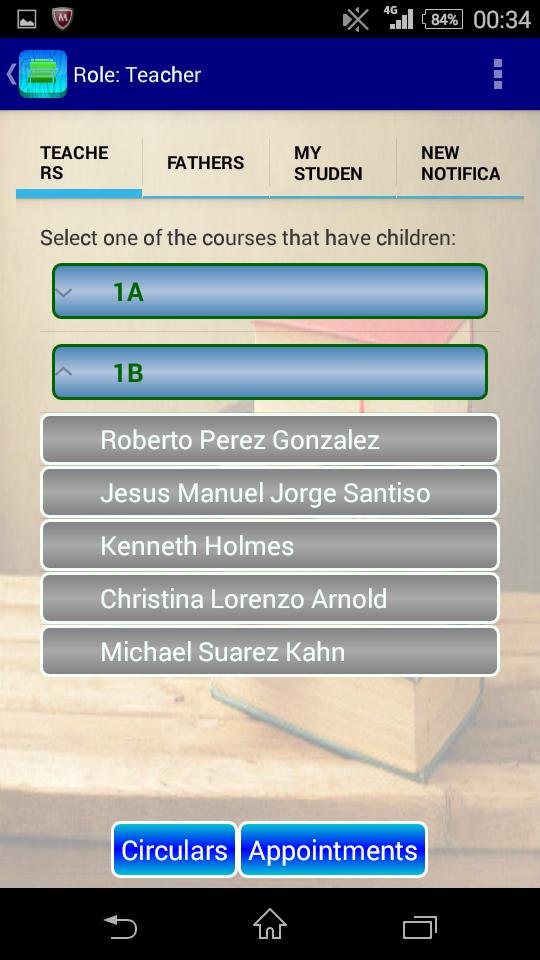
\includegraphics[scale=0.2]{Imagenes/App/profeProfe}
				\caption{Lista de contacto de profesores para el perfil de profesor.}
				\label{fig:profeProfe}
			\end{figure}
		
		\subsection{Lista de contactos: Padres (ExpandableFathersActivity)}
		
			En la figura \ref{fig:profePadre} se puede observar los contactos que son padres de alumnos a los que imparte clase. Al seleccionar cualquiera de los contactos se podrá comunicar de forma directa con mensajes tipo chat (sección \ref{sec:chat}). Al hacer una selección larga podrá ver la información del contacto (sección \ref{sec:data}).
			
			\begin{figure}[h !]
				\centering
				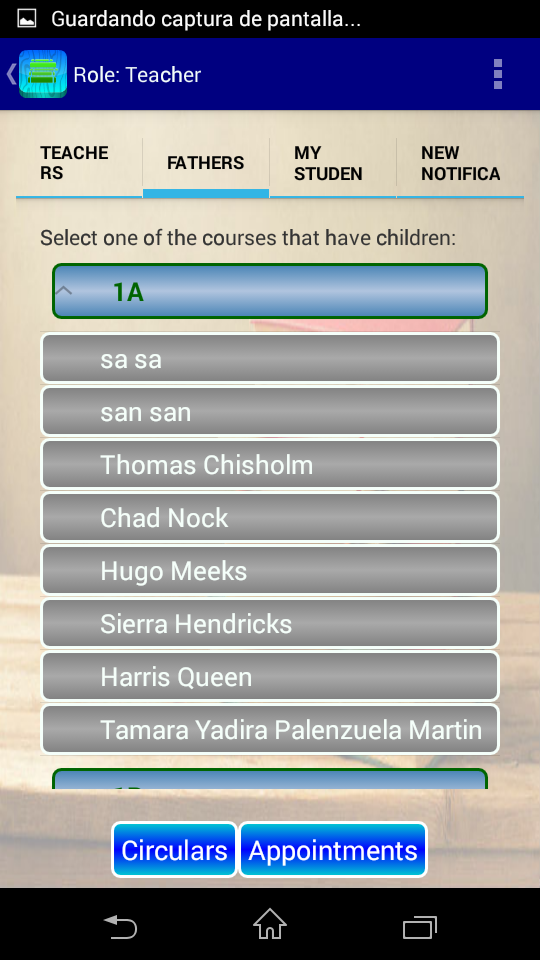
\includegraphics[scale=0.2]{Imagenes/App/profePadre}
				\caption{Lista de contacto de padres para el perfil de profesor.}
				\label{fig:profePadre}
			\end{figure}
		
		\subsection{Lista de contactos: Alumnos (ExpandableAlumnosActivity)}
		
			En esta pantalla (figura \ref{fig:profeAlu}) se mostrarán los alumnos a los que un profesor imparte clase. Al seleccionar cualquiera de los contactos se podrá comunicar de forma directa con mensajes tipo chat (sección \ref{sec:chat}). Al hacer una selección larga podrá ver la información del contacto (sección \ref{sec:data}).
		
			\begin{figure}[h !]
				\centering
				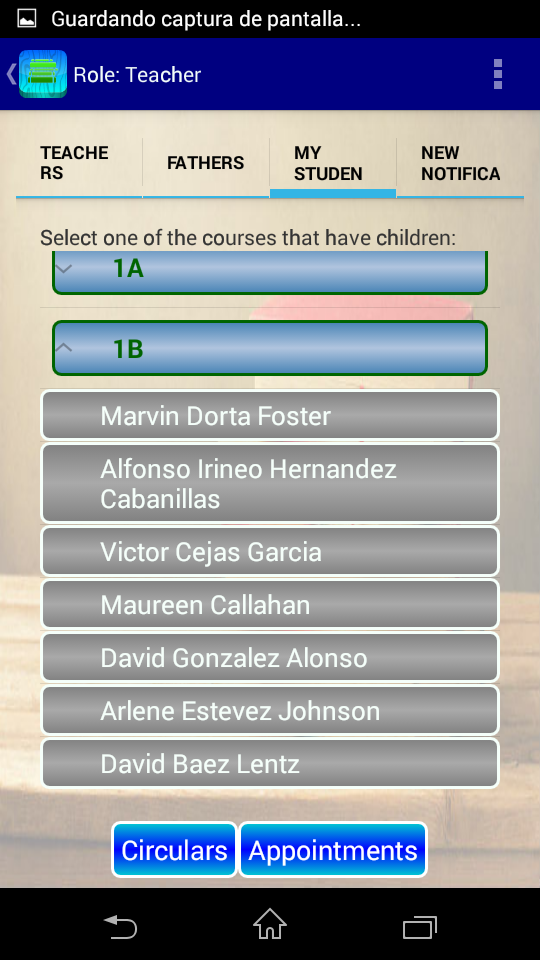
\includegraphics[scale=0.2]{Imagenes/App/profeAlu}
				\caption{Lista de contacto de alumnos para el perfil de padre.}
				\label{fig:profeAlu}
			\end{figure}
		
	\section{Notificaciones (notificationsActivity)} \label{sec:notifications}
	
		En la figura \ref{fig:notifications} se puede observar todas las notificaciones que reciben los usuarios. Estas son recuperadas y eliminadas de la base de datos en {\it Friebase}. La notificación muestra el nombre del remitente y el número de mensajes que ha enviado y que el usuario tiene sin leer. Se clasifican por colores según el perfil del usuario que las manda.
		Al seleccionar cualquiera se podrá comunicar de forma directa con mensajes tipo chat (sección \ref{sec:chat}) con el remitente.
	
		\begin{figure}[h !]
			\centering
			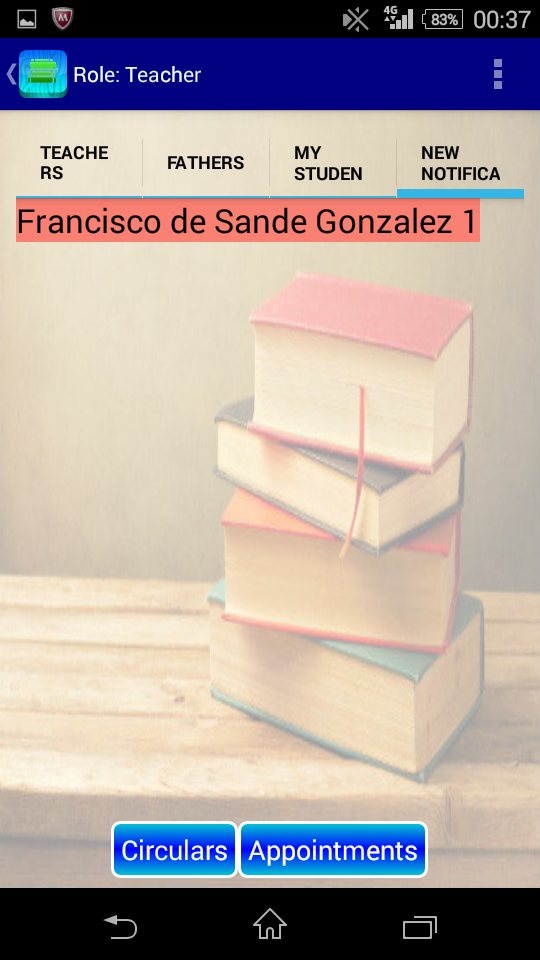
\includegraphics[scale=0.2]{Imagenes/App/Notifications}
			\caption{Notificaciones recibidas por los usuarios.}
			\label{fig:notifications}
		\end{figure}
	
	\section{Chat (ChatActivity)} \label{sec:chat}
	
		En esta pantalla (figura \ref{fig:chat}) obtenemos mensajería directa tipo chat con cualquiera de los contactos del usuario. Estos mensajes se guardan en la base de datos de {\it Firebase} de donde son recuperados y eliminados. También se guardan en una base de datos local, almacenada en el dispositivo. Si accedemos a las opciones podemos vaciar la conversación.
	
		\begin{figure}[h !]
			\centering
			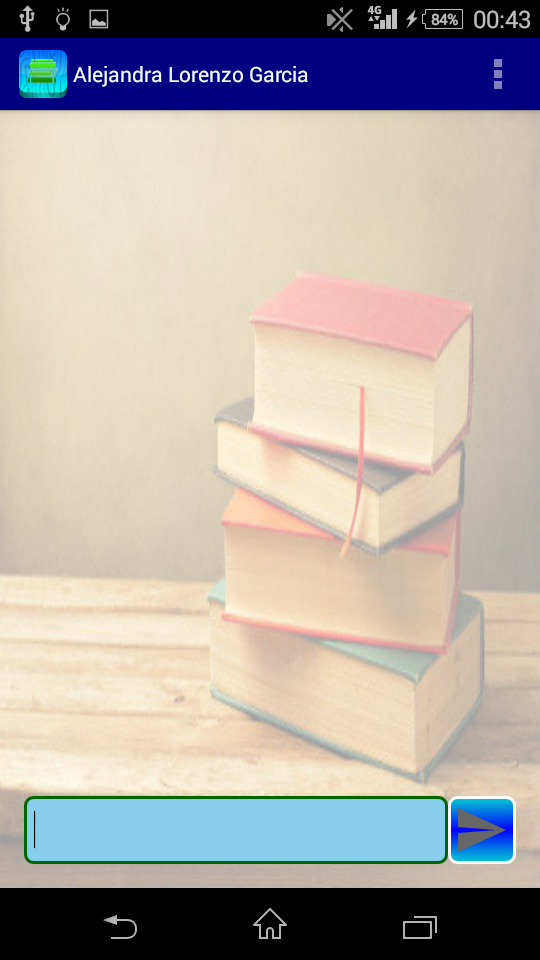
\includegraphics[scale=0.2]{Imagenes/App/chat}
			\caption{Mensajería tipo chat.}
			\label{fig:chat}
		\end{figure}
	
	\section{Mis Datos (MyDataActivity)} \label{sec:myData}
	
		En la figura \ref{fig:myData} se puede observar que el usuario puede ver los datos con los que se registró. Al seleccionar el botón modificar, podrá cambiar sus datos salvo el D.N.I y el correo electrónico. Si selecciona guardar se modificará la base de datos en el proveedor de servicios.
		Su selecciona dar de baja su cuenta, se borrará la información que hay en {\it Firebase}. También puede cambiar su contraseña con el botón destinado a ello (sección \ref{sec:changePassword}).
		
		\begin{figure}[h !]
			\centering
			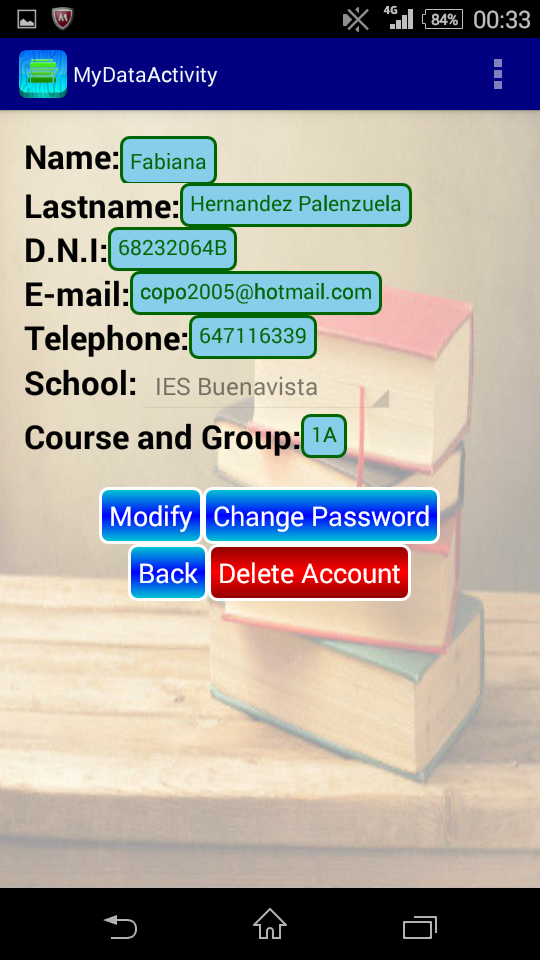
\includegraphics[scale=0.2]{Imagenes/App/myData}
			\caption{Datos del usuario.}
			\label{fig:myData}
		\end{figure}
	
	\section{Cambio de Contraseña (ChangePasswordactivity)} \label{sec:changePassword}
	
		En la pantalla de cambio de contraseña el usuario podrá cambiar su contraseña introduciendo su correo electrónico y contraseña antigua. También deberá seleccionar una nueva contraseña y repetirla. Si desea hacer el cambio permanente solo deberá accionar el botón guardar.
	
		\begin{figure}[h !]
			\centering
			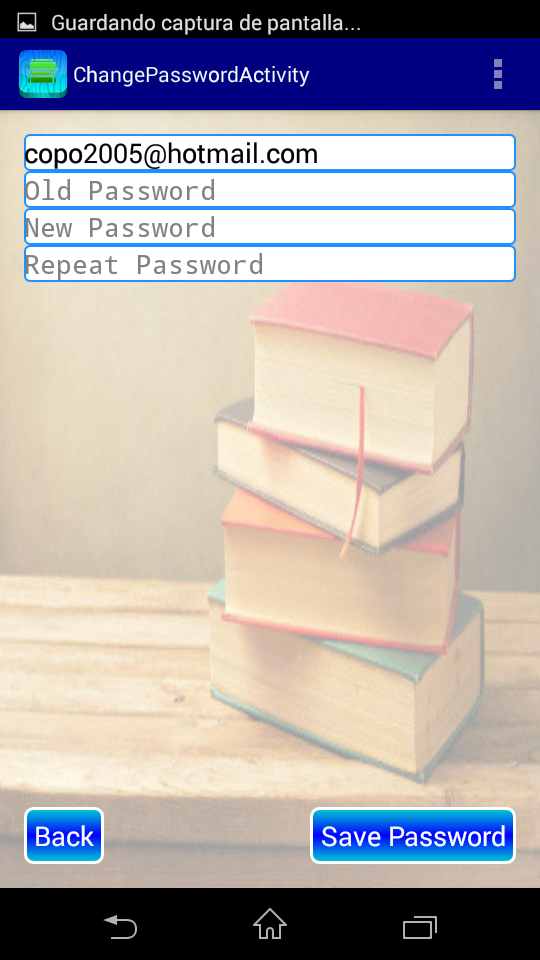
\includegraphics[scale=0.2]{Imagenes/App/changePassword}
			\caption{Cambio de contraseña.}
			\label{fig:changePassword}
		\end{figure}
	
	\section{Circulares (CircularesActivity)} \label{sec:circulares}
	
		En esta pantalla (figura \ref{fig:circulares}) se podrá mandar un mismo mensaje a una o varias clases, ya sean alumnos o padres. Al seleccionar el botón enviar, se mandará el mismo mensaje a cada uno de los alumnos que pertenezca a la clase seleccionada.
	
		\begin{figure}[h !]
			\centering
			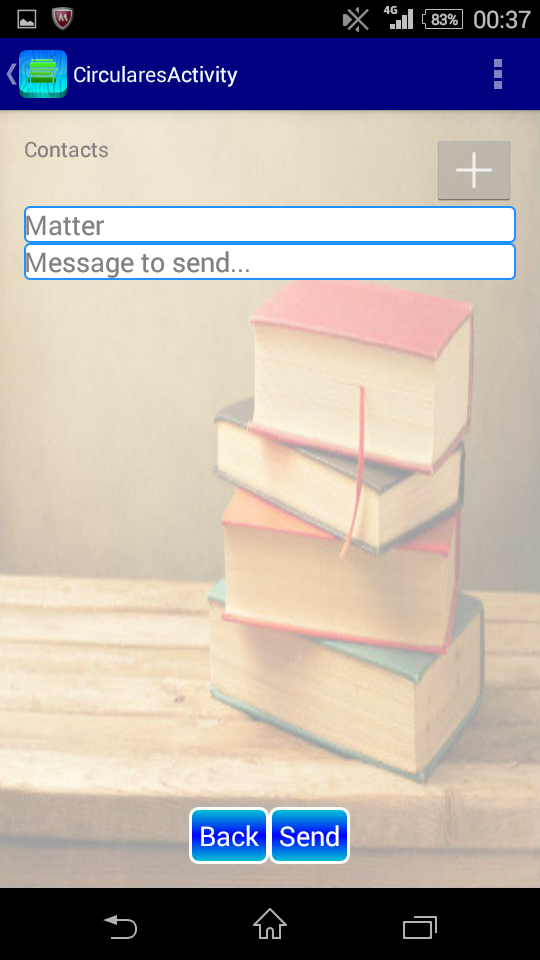
\includegraphics[scale=0.2]{Imagenes/App/Circulares}
			\caption{Pantalla de circulares.}
			\label{fig:circulares}
		\end{figure}
		
		En la figura \ref{fig:selectClass} se puede observar cómo se seleccionan las clases.
		
		\begin{figure}[h !]
			\centering
			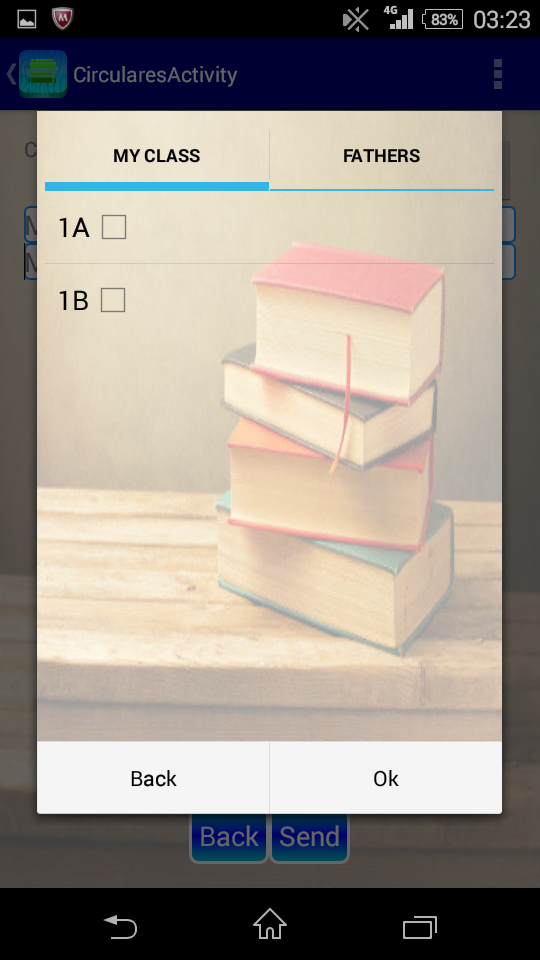
\includegraphics[scale=0.2]{Imagenes/App/selectClass}
			\caption{Pantalla de circulares, seleccionar clase.}
			\label{fig:selectClass}
		\end{figure}
	
	\section{Citas} \label{sec:dates}
		Esta funcionalidad (figura \ref{fig:addEvent}) usa el calendario del dispositivo. Lanza la actividad que permite añadir eventos. Viene implementado en el {\it sistema operativo}.
		Se introducen los datos en los campos correspondientes y luego se selecciona guardar. Se puede elegir el calendario en el que guardar el evento, en el dispositivo o en el de {\it Google}.
		
			\begin{figure}[h !]
				\centering
				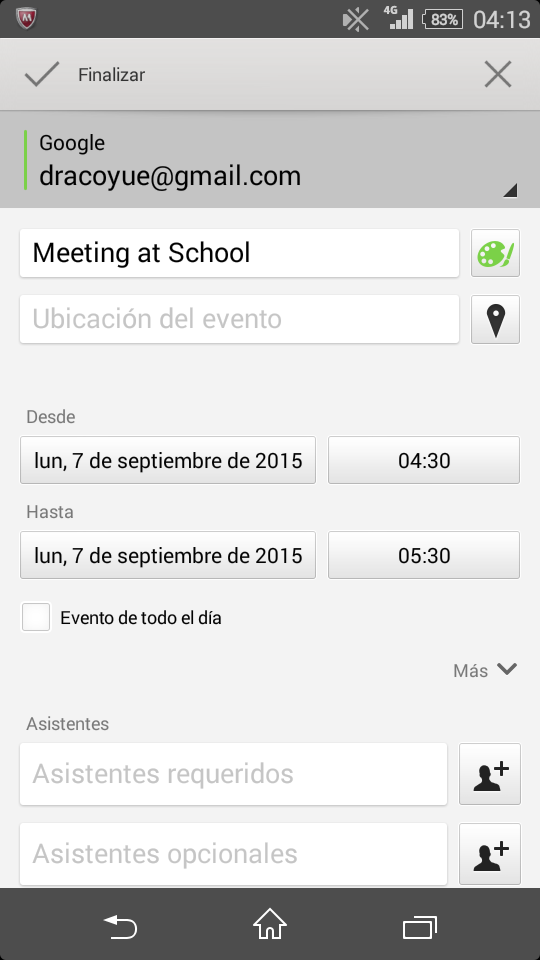
\includegraphics[scale=0.2]{Imagenes/App/addEvent}
				\caption{añadir evento al calendario.}
				\label{fig:addEvent}
			\end{figure}
	
	\section{Datos del contacto (DataActivity)} \label{sec:data}
	
		En esta pantalla (figura \ref{fig:data}) se muestran los datos de cualquier contacto del usuario.
		
		\begin{figure}[h !]
			\centering
			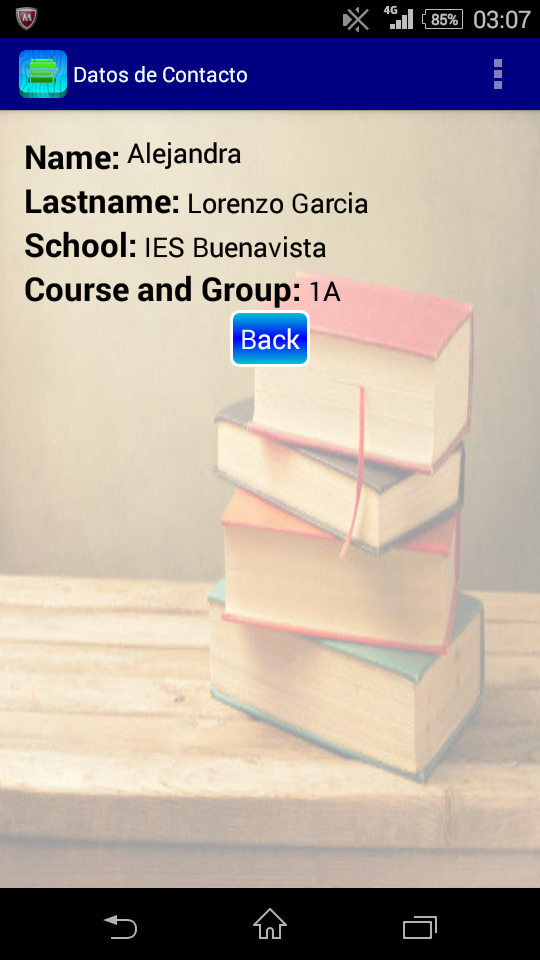
\includegraphics[scale=0.2]{Imagenes/App/dataContact}
			\caption{Pantalla de datos de un contacto.}
			\label{fig:data}
		\end{figure} %A mandar
	%
% ---------------------------------------------------
%
% Trabajo de Final de Grado:
% Author: Gonzalo Jesús García Martín <dracoyue@gmail.com>
% Capítulo: Introducción
% Fichero: Cap7_DesarrolloApp.tex
%
% ----------------------------------------------------
%

\cleardoublepage
\chapter{Desarrollo de la Aplicación}
\label{chap:developing}

	En este capítulo se expondrá la implementación de las clases más relevantes para la aplicación.
	Sería demasiado extenso explicar en profundidad cada uno de los elementos que componen la aplicación.
	La figura \ref{fig:ClassDiagram} presenta un diagrama de clases de \CollegeApp\ mientras que en el apéndice \ref{chap:activitiesdiagram} muestra el diagrama de actividades(figura \ref{fig:ActivitiesDiagram}).
	
	\bigskip
	Todo el código de \CollegeApp\ \cite{28:mirepo:online} está disponible públicamente en el repositorio de github.
	
	\section{Clase {\ttfamily Student}} \label{sec:Student}
	
		Esta es la clase encargada de almacenar los datos de los alumnos que se obtienen desde el {\it proveedor de servicios}.
		El constructor obtiene los datos desde un {\it HashMap} \cite{10:hashmap:online} que es el objeto que devuelven las consultas a la base de datos. También se ha implementado la interfaz {\it Parcelable} \cite{11:parcelable:online} que es la que permite compartir objetos de una clase entre {\it Activities}. 
		En el listado \ref{code:StudentJava} se puede observar la implementación de la clase.
		
		\lstinputlisting[float=h!, language=Java,caption={Ejemplo de la clase Student.},label={code:StudentJava}]{Code/Student.java}
		
		\bigskip
		Entre las líneas 19 y 25 se observa el método {\ttfamily writeToParcel()}, que implementa la forma de introducir datos de un objeto de la clase {\it Parcelable}.
		
		El método {\ttfamily readFromParcel()} (líneas de la 26 a la 30) muestra como se obtienen los datos de esta clase. En este método, los atributos deben estar en el mismo orden que el en {\ttfamily writeToParcel()}.
		
		De la línea 31 a la 36, se se muestra como crear un objeto de la clase {\it Parcelable}.
	
	\section{Clase {\ttfamily Father}}
	
		Esta es la clase encargada de almacenar los datos de los usuarios con el rol de padre que se obtienen desde la {\it nube}.
		Los atributos de la clase son: name, lastname, mail, telephone, dni, childrens ({\it ArrayList} \cite{12:arraytist:online} de la clase {\ttfamily Student} que son hijos del usuario) y rol.
		Funciona igual que la clase {\ttfamily Student} (sección \ref{sec:Student}).
				
		\bigskip
		Los métodos más importantes en esta clase son {\ttfamily getClassrooms()} que devuelve un ArrayList con las clases en las que están registrados los hijos y {\ttfamily getSchools()} que devuelve otro ArrayList con los colegios a los que asisten los hijos.
	
	\section{Clase {\ttfamily Teacher}}
	
		Esta es la clase encargada de almacenar los datos de los usuarios con el perfil de profesor que se obtienen desde la {\it nube}.
		Los atributos de la clase son name, lastname, mail, telephone, dni y rol.
		Funciona igual que la clase {\ttfamily Student} (sección \ref{sec:Student}).
		
		El constructor obtiene los datos desde un {\it HashMap} \cite{10:hashmap:online} que es el objeto que devuelven las consultas a la base de datos. También se ha implementado la interfaz {\it Parcelable} \cite{11:parcelable:online} que es la que permite compartir objetos de una clase entre {\it Activities}. 
		
	\section{Clase {\ttfamily Message}}
	
		Esta es la clase encargada de almacenar los datos de los mensajes que se obtienen desde la {\it nube}.
		A continuación se enumeran los atributos de la clase:
		
		\begin{itemize}
			\setlength{\itemsep}{1pt}
			\setlength{\parskip}{0pt}
			\setlength{\parsep}{0pt}
			\item {\it dniRemitter}: D.N.I del remitente del mensaje.
			\item {\it remitter}: Nombre del remitente del mensaje, se usa para mostrar el nombre en {\ttfamily NotificationsActivity} (sección \ref{sec:notifications}).
			\item {\it message}: Mensaje que envían los usuarios.
			\item {\it rolRemmiter}: Perfil del remitente, se usa para colorear las notificaciones.
			\item {\it date}: fecha del mensaje.
			\item {\it destinatario}: Este campo solo está presente en la base de datos. Se usa para recuperar los mensajes.
		\end{itemize}
		
		Funciona igual que la clase {\ttfamily Student} (sección \ref{sec:Student}).
		
	\section{Clase {\ttfamily MessageSQLHelper}}
		Cada uno de los mensaje enviados entre los usuarios está almacenado en el dispositivo, en una base de datos local {\it SQLite}\cite{13:sqlite:online}.
		
		\bigskip
		La tabla {\ttfamily messages} almacena los mensajes que se envían desde el dispositivo. Sus atributos son:
		
		\begin{itemize}
			\setlength{\itemsep}{1pt}
			\setlength{\parskip}{0pt}
			\setlength{\parsep}{0pt}
			\item {\it idConversation}: Identificación de la conversación.
			\item {\it dniRemitter}: D.N.I del remitente.
			\item {\it remitter}: Nombre del remitente.
			\item {\it message}: Mensaje. 
			\item {\it day, month, year, hour, minute}: Datos del envío del mensaje.
		\end{itemize}
		
		\bigskip
		La tabla {\ttfamily conversations} almacena el identificador de la conversación entre dos usuarios.
		Sus atributos son:
		
		\begin{itemize}
			\setlength{\itemsep}{1pt}
			\setlength{\parskip}{0pt}
			\setlength{\parsep}{0pt}
			\item {\it id}: Identificación de la conversación.
			\item {\it dniSender}: D.N.I del usuario que envía el mensaje.
			\item {\it dniRemitter}: D.N.I del remitente.
		\end{itemize}
		
		En el listado \ref{code:MessageDBJava} se muestra la implementación de la clase.
		
		\lstinputlisting[float = h!,language=Java,caption={Ejemplo de la clase MessageSQLHelper.},label={code:MessageDBJava}]{Code/MessageSQLHelper.java}
		
		Desde la línea 6 hasta la 24, se muestra el método {\ttfamily onCreate()} donde se crean las las tablas descritas anteriormente. Para cada tabla se crea una variable de tipo cadena ({\it String}) con la definición cada uno de sus atributos. Después se ejecuta la función {\ttfamily execSQL()} y se le pasa como parámetro la variable creada.
		
	\section{\ttfamily TabActivityes}
		Cuando el usuario accede a \CollegeApp\ se le muestra una pantalla con pestañas donde se hallan sus contactos. Cada pestaña es una actividad distinta a causa del problema \ref{prob:8}. Al cambiar de pestaña se cambia de actividad y la consulta deja de ejecutarse.
		Esta solución ha sido la principal forma de construir la aplicación y solventar los problemas principales.
		
		\bigskip
		En el listado \ref{code:studentTab} se muestra como se crean las pestañas en las que se mostrarán las listas de contactos. En la línea 5 se obtiene el elemento donde se añadirán las pestañas, llamado {\ttfamily TabHost} \cite{25:tabhost:online}. Se crea el objeto que lanzará la actividad deseado (línea 10) y se añade al {\ttfamily TabHost}.
		
		\lstinputlisting[float = h!,language=Java,caption={Ejemplo de la clase StudentTabActivity.},label={code:studentTab}]{Code/StudentTabActivity.java}
		
		\bigskip
		La clase {\ttfamily StudentActivity} (listado \ref{code:studentActivity}) muestra un ejemplo de la interacción con la base de datos. En la línea 8 se puede ver la consulta que obtiene los alumnos que asisten a la misma clase que el usuario. A esta consulta se le añade un oyente que conecta con la base de datos y espera por si se modifican los datos. Se crea el objeto de la clase correspondiente en la línea 13 y se añade a un {\it ArrayList} con el que se rellenará la lista de contactos.
		
		\lstinputlisting[float = h!,language=Java,caption={Ejemplo de la clase StudentActivity.},label={code:studentActivity}]{Code/StudentActivity.java}
	
		\bigskip
		En listado \ref{code:StudentRegisterJava} se muestra como se envía información a la base de datos. Al registrar al usuario se observa como existe una función que comprueba que todos los datos del formulario sean correctos (línea 7, {\ttfamily haveEmptyFields()}). Para permitir el acceso a \CollegeApp\ hay que crear al usuario como se muestra en la línea 8. Si se crea al usuario de forma satisfactoria, se procede a enviar la información a {\it Firebase}. Se crea un {\it HashMap} y se introducen los datos del usuario con el método {\ttfamily put()} (líneas 11 a 14). Se selecciona un identificador único (línea 15) y se envía a la base de datos. {\ttfamily studentRef} es la referencia a la tabla en la que se introducirán los datos, {\ttfamily child(uuid)} es la función que selecciona la fila correspondiente al usuario y {\ttfamily setValue(aluMap)} permite almacenar los datos que contiene el {\it HashMap} (línea 16).
		
		\lstinputlisting[float = h!,language=Java,caption={Ejemplo de la clase StudentRegisterActivity.},label={code:StudentRegisterJava}]{Code/StudentRegisterActivity.java}
	
	\section{Problemas}
		Al diseñar una aplicación siempre surgen problemas inesperados en los que hay que agudizar el ingenio para resolverlos.
		
		En este capítulo se expondrán los problemas ocurridos a la hora de programar, se irán enumerando y explicando la forma de resolverlos.
		
		\begin{enumerate}
			\item {\bf Android Studio no render target}
			\begin{itemize}
				\item {\bf Solución}:
				\begin{enumerate}
					\item Asegúrese de que hay un dispositivo real o virtual seleccionado.
					\item Tener una versión de {\it Android} seleccionada.
					\item Versiones necesarias para el desarrollo dela aplicación en {\it Android} instaladas.
					\item Crear un nuevo {\it Dispositivo Virtual} ({\it AVD}).
					% Meter dibujo de AVD
					\item Reiniciar Android Studio.
				\end{enumerate}
			\end{itemize}
			
			\item {\bf Fallo al encontrar com.android.support:appcompat-v7:16.+}
			\begin{itemize}
				\item {\bf Solución}: Actualizar en las dependencias del archivo {\ttfamily build.gradle}, en el directorio {\ttfamily app} que está en la raíz del proyecto, la librería deberá ser la última versión disponible. Este cambio se realiza de forma manual.
			\end{itemize}
			
			\item {\bf Fallo al encontrar Java}
			\begin{itemize}
				\item {\bf Solución}: Si java ya está instalado, averigüe el directorio. Una vez hecho esto necesita volver a establecer la variable de ámbito indicando la localización correcta. Seleccione {\ttfamily Iniciar \textgreater Equipo \textgreater Propiedades \textgreater Configuración Avanzada del Sistema}.
				Entonces abra la pestaña {\ttfamily Opciones Avanzadas \textgreater Variables de Entorno} y añada una nueva variable de sistema llamada {\ttfamily JAVA\_HOME} que  tenga como valor la dirección del directorio donde tenga instalado el {\it JDK}, por ejemplo, {\ttfamily C:{\textbackslash}Program Files{\textbackslash}Java{\textbackslash}jdk1.7.0\_21}. 
			\end{itemize}
			\item {\bf Duplicidad en las dependencias de los paquetes}
			\begin{itemize}
				\item {\bf Solución}: Si se tiene un error de compilación sobre archivos duplicados, se puede excluir esos ficheros añadiendo la directiva {\ttfamily packagingOptions} al archivo {\ttfamily build.gradle} que está en el directorio {\ttfamily app}. Como se muestra en el listado \ref{code:duplicidadbuild}.
				
				\lstinputlisting[float = h!, language=Java,caption={Solución a la duplicidad en {\ttfamily build.gradle}.}, label={code:duplicidadbuild}]{Code/duplicidadbuild.gradle}
			\end{itemize}
			
			\item {\bf Fallo al encontrar android.support.v13}
			\begin{itemize}
				\item {\bf Solución}: Añadir en las dependencias del archivo {\ttfamily build.gradle}, en el directorio {\ttfamily app} que está en la raíz del proyecto, la orden {\ttfamily compile 'com.android.support:support-v13:21.+'} de forma manual. Como se puede analizar en el listado \ref{code:supportv13}.
				
				\noindent
				\lstinputlisting[float = h!, language=Java,caption={Solución al problema supportV13.},label={code:supportv13}]{Code/support13build.gradle}
			\end{itemize}
			
			\item {\bf Arregle Gradle (Fix Gradle)}
			\begin{itemize}
				\item {\bf Solución}:
				\begin{enumerate}
					\item En el archivo {\ttfamily buil.gradle} que está en el directorio raíz del proyecto, añadir la dependencia de forma manual: {\ttfamily classpath 'com.android.tools.build:gradle:1.0.0' }. Listado \ref{code:buildGradle}.
					\item En el archivo {\ttfamily buil.gradle}, que está en el directorio {\ttfamily app} en la raíz del proyecto, añadir dentro de {\ttfamily release} de forma manual, listado \ref{code:appBuildGradle}.
					
				\end{enumerate}
				\noindent
				\lstinputlisting[float = h!,language=Java,caption={Solución en {\ttfamily build.gradle}.},label={code:buildGradle}]{Code/buildgradle.gradle}
				\lstinputlisting[float = h,language=Java,caption={Solución en {\ttfamily app/build.gradle}.},label={code:appBuildGradle}]{Code/appbuildgradle.gradle}
			\end{itemize}
			
			\item {\bf SDK no encontrado}
			\begin{itemize}
				\item {\bf Solución}: Si AndroidStudio no encuentra el {\it SDK} y está instalado seleccionar {\ttfamily Windows \textgreater Preferencias \textgreater Android \textgreater Localización SDK} y establecer el directorio donde se tiene instalado.
			\end{itemize}
			
			\item {\bf Consultas a la espera de cambios en los datos} \label{prob:8}
			\begin{itemize}
				\item {\bf Solución}: Existen dos tipos de consultas en {\it Firebase}, las que devuelven un solo resultado ({\ttfamily addListenerForSingleValueEvent()}) y las que devuelven varios resultados ({\ttfamily addChildEventListener()}). Éstas últimas se quedan esperando por si se modifican datos de la base de datos.
				La solución sería remover el {\ttfamily listener} al final de su uso ({\ttfamily ref.removeEventListener(originalListener);}) o tener una sola consulta del segundo tipo por actividad.
			\end{itemize}
		\end{enumerate} %A mandar
	%
% ---------------------------------------------------
%
% Trabajo de Final de Grado:
% Author: Gonzalo Jesús García Martín <dracoyue@gmail.com>
% Capítulo: Objetivos
% Fichero: Cap5_Problemas.tex
%
% ----------------------------------------------------
%

\cleardoublepage
\chapter{Problemas}
\label{chap:troubles}

	Al diseñar una aplicación siempre surgen problemas inesperados en los que hay que agudizar el ingenio para resolverlos.

	En este capítulo se expondrán los problemas ocurridos a la hora de programar, se irán enumerando y explicando la forma de resolverlos.

	\begin{enumerate}
		\item {\bf Android Studio no render target}
			\begin{itemize}
				\item {\bf Solución}:
					\begin{enumerate}
						\item Asegúrese de que hay un dispositivo real o virtual seleccionado.
						\item Tener una versión de {\it Android} seleccionada.
						\item Versiones necesarias para el desarrollo dela aplicación en {\it Android} instaladas.
						\item Crear un nuevo {\it Dispositivo Virtual} ({\it AVD}).
						% Meter dibujo de AVD
						\item Reiniciar Android Studio.
					\end{enumerate}
			\end{itemize}
		
		\item {\bf Fallo al encontrar com.android.support:appcompat-v7:16.+}
			\begin{itemize}
				\item {\bf Solución}: Actualizar en las dependencias del archivo {\ttfamily build.gradle}, en el directorio {\ttfamily app} que está en la raíz del proyecto, la librería deberá ser la última versión disponible. Este cambio se realiza de forma manual.
			\end{itemize}
		
		\item {\bf Fallo al encontrar Java}
			\begin{itemize}
				\item {\bf Solución}: Si java ya está instalado, averigüe el directorio. Una vez hecho esto necesita volver a establecer la variable de ámbito indicando la localización correcta. Seleccione {\ttfamily Iniciar \textgreater Equipo \textgreater Propiedades \textgreater Configuración Avanzada del Sistema}.
				Entonces abra la pestaña {\ttfamily Opciones Avanzadas \textgreater Variables de Entorno} y añada una nueva variable de sistema llamada {\ttfamily JAVA\_HOME} que  tenga como valor la dirección del directorio donde tenga instalado el {\it JDK}, por ejemplo, {\ttfamily C:{\textbackslash}Program Files{\textbackslash}Java{\textbackslash}jdk1.7.0\_21}. 
			\end{itemize}
		\item {\bf Duplicidad en las dependencias de los paquetes}
			\begin{itemize}
				\item {\bf Solución}: Si se tiene un error de compilación sobre archivos duplicados, se puede excluir esos ficheros añadiendo la directiva {\ttfamily packagingOptions} al archivo {\ttfamily build.gradle} que está en el directorio {\ttfamily app}. Como se puede observar en el listado \ref{code:duplicidadbuild}.
				
				\lstinputlisting[float = h!, language=Java,caption={Solución a la duplicidad en {\ttfamily build.gradle}.}, label={code:duplicidadbuild}]{Code/duplicidadbuild.gradle}
			\end{itemize}
			
		\item {\bf Problemas con import android.support.v13}
			\begin{itemize}
				\item {\bf Solución}: Añadir en las dependencias del archivo {\ttfamily build.gradle}, en el directorio {\ttfamily app} que está en la raíz del proyecto, la orden {\ttfamily compile 'com.android.support:support-v13:21.+'} de forma manual. Como se puede analizar en el listado \ref{code:supportv13}.
				
				\noindent
				\lstinputlisting[float = h!, language=Java,caption={Solución al problema supportV13.},label={code:supportv13}]{Code/support13build.gradle}
			\end{itemize}
			
		\item {\bf Problemas con Gradle}
			\begin{itemize}
				\item {\bf Solución}:
					\begin{enumerate}
						\item En el archivo {\ttfamily buil.gradle} que está en el directorio raíz del proyecto, añadir la dependencia de forma manual: {\ttfamily classpath 'com.android.tools.build:gradle:1.0.0' }. Listado \ref{code:buildGradle}.
						\item En el archivo {\ttfamily buil.gradle}, que está en el directorio {\ttfamily app} en la raíz del proyecto, añadir dentro de {\ttfamily release} de forma manual, listado \ref{code:appBuildGradle}.
							
					\end{enumerate}
					\noindent
					\lstinputlisting[float = h!,language=Java,caption={Solución en {\ttfamily build.gradle}.},label={code:buildGradle}]{Code/buildgradle.gradle}
					\lstinputlisting[float = h,language=Java,caption={Solución en {\ttfamily app/build.gradle}.},label={code:appBuildGradle}]{Code/appbuildgradle.gradle}
			\end{itemize}
		
		\item {\bf SDK no encontrado}
			\begin{itemize}
				\item {\bf Solución}: Si AndroidStudio no encuentra el {\it SDK} y está instalado seleccionar {\ttfamily Windows \textgreater Preferencias \textgreater Android \textgreater Localización SDK} y establecer el directorio donde se tiene instalado.
			\end{itemize}
			
		\item {\bf Consultas Asíncronas}
			\begin{itemize}
				\item {\bf Solución}: Existen dos tipos de consultas en {\it Firebase}, las que devuelven un solo resultado ({\ttfamily addListenerForSingleValueEvent()}) y las que devuelven varios resultados ({\ttfamily addChildEventListener()}). Éstas últimas se quedan esperando por si se modifican datos de la base de datos.
				La solución sería removerlo al final de su uso ({\ttfamily ref.removeEventListener(originalListener);}) o tener una sola consulta del segundo tipo por actividad.
			\end{itemize}
	\end{enumerate} %A mandar
	%
% ---------------------------------------------------
%
% Trabajo de Final de Grado:
% Author: Gonzalo Jesús García Martín <dracoyue@gmail.com>
% Capítulo: Fases
% Fichero: Cap8_Conclusiones_LineasFuturas.tex
%
% ----------------------------------------------------
%

\cleardoublepage
\chapter{Conclusiones y Trabajos futuros}
\label{chap:conclusions}

	En este capítulo se revisarán los posibles trabajos por hacer en \CollegeApp, ya que toda aplicación debe estar dispuesta a ser mejorada. También se hablará de las conclusiones y experiencias adquiridas a lo largo de la realización de este proyecto que ha sido especialmente enriquecedor.

	\section{Trabajos futuros}
	
		Se contemplarán casos de uso que no se han implementado a la hora de crear la aplicación. Algunos perfiles ordenados según su dificultad de desarrollo son:
		
		\begin{itemize}
			\item Padres con hijos en distintos centros: en algún momento, alumnos con el mismo padre, madre o tutor legal podrían asistir a centros escolares distintos.
			\item Usuarios con distintos perfiles en el mismo colegio, por ejemplo, un profesor que imparta clases en el colegio al que asiste su hijo.
			\item Profesores que trabajan en más de un centro escolar: En este caso se contemplará profesores que impartan clases en más de un colegio.
		\end{itemize}
		
		También se contemplarán otras funcionalidades, estas están ordenadas en función de su dificultad de implementación:
		\begin{itemize}
			\item Búsqueda de contactos: El usuario podrá buscar un contacto concreto introduciendo su nombre en un cuadro de búsqueda.
			\item Envío de boletines de notas: Proporcionará a los profesores la funcionalidad de enviar las notas de sus alumnos a los padres de éstos.
			\item Envío de archivos a través de la aplicación: Permitirá a los usuarios compartir archivos.
		\end{itemize}
		
	\section{Conclusiones}
		La realización de este proyecto nos ha permitido aplicar los conocimientos técnicos obtenidos durante los años de estudio, permitiendo la asimilación real de las competencias necesarias y la adquisición nuevos conocimientos.
		Esta experiencia da a conocer el grado de implicación que conlleva crear una aplicación totalmente funcional en un ámbito real. El análisis de otras aplicaciones similares permite concretar el estado del mercado con respecto al tipo de aplicación creada.
		
		\bigskip
		Programar una aplicación puede parecer sencillo, pero conlleva dedicación, tiempo, trabajo y esfuerzo. %A mandar
	%
% ---------------------------------------------------
%
% Trabajo de Final de Grado:
% Author: Gonzalo Jesús García Martín <dracoyue@gmail.com>
% Capítulo: Fases
% Fichero: Cap9_Cap8English.tex
%
% ----------------------------------------------------
%

\cleardoublepage
\chapter{Conclusions and Future works}
\label{chap:futureLines}

	This chapter reviews different ways to enhance \CollegeApp, since every application must be willing to be improved. It will also discuss the conclusions and lessons learned along the realization of this project that has been especially rewarding.

	\section{Future works}
	
		Use cases that have not been implemented when creating the application behold. Some profiles are sorted according to their difficulty:
		
		\begin{itemize}
			\item Parents with children in different schools: At some point, students with the same parent or guardian attend different schools.
			\item Users with different profiles on the same school, for example, a school teacher in the school that your child attends.
			\item Teachers working in more than one school: In this case teachers to teach classes in more than one school will be contemplated.
		\end{itemize}
		
		Other features will also be envisaged, these are sorted according to their difficulty of implementation:
		
		\begin{itemize}
			\item Finding contacts.
			\item Sending report cards.
			\item Sending files through the application.
		\end{itemize}
	
	\section{Conclusions}
		The realization of this project will apply the expertise gained during the years of study, allowing real assimilation of the necessary skills and acquire new knowledge.
		This experience discloses the level of involvement that involves creating a fully functional application in a real environment. The analysis of other similar applications can realize the state of the market for the type of application built.
		
		\bigskip
		An application program may seem simple, but it takes dedication, time and hard work. %A mandar
	%
% ---------------------------------------------------
%
% Trabajo de Final de Grado:
% Author: Gonzalo Jesús García Martín <dracoyue@gmail.com>
% Capítulo: Objetivos
% Fichero: Cap10_Presupuesto.tex
%
% ----------------------------------------------------
%

\cleardoublepage
\chapter{Presupuesto}
\label{chap:budget}

	Este presupuesto está dirigido a empresas, principalmente a colegios que deseen adquirir \CollegeApp. Se ha desglosado en el presupuesto la cantidad de horas de análisis y de implementación que se han empleado en cada funcionalidad de la aplicación.
		
		\begin{figure}[h !]
			\centering
			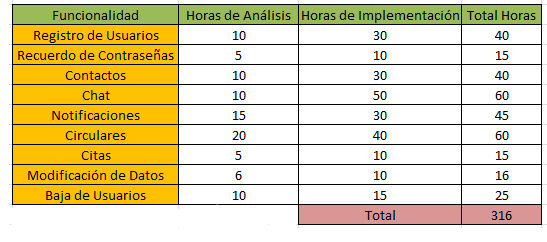
\includegraphics{horas}
			\caption{Horas empleadas en el desarrollo de la aplicación}
			\label{fig:presupuesto}
		\end{figure}
		
		La cantidad de horas invertidas en la aplicación son {\bf 316 horas}. La tarifa de desarrollo establecida en este proyecto es de {\bf 3.5 euros la hora} lo cual conduce a un total de {\bf 1106 euros de honorarios}. A lo cual hay que agregarle la adquisición de dos dispositivos de gama media a {\bf 119 euros cada uno} para pruebas con la aplicación.
		
		\bigskip
		Dicho esto, la aplicación tiene un coste de {\bf \large 1334 euros}. %A Hacer----------------------------------------
	
	
%%%%%%%%%%%%%%%%%%%%%%%%%%%%%%%%%%%%%%%%%%%%%%%%%%%%%%%%%%%%%%%%%%%%%%%%%%%%%%%%%%%%%%%%%%%%%%%%
%%%%%%Apéndices%%%%%%
	\appendix
	%\appendixname
	%
% ---------------------------------------------------
%
% Trabajo de Final de Grado:
% Author: Gonzalo Jesús García Martín <dracoyue@gmail.com>
% Capítulo:  diagrama de Clases
% Fichero: ApendiceA_diagramaClases.tex
%
% ----------------------------------------------------
%

\cleardoublepage
\chapter{Diagrama de Clases}
\label{chap:classdiagram}

Se puede ver una imagen del diagrama de clases:

\begin{figure}[h !]
	\centering
	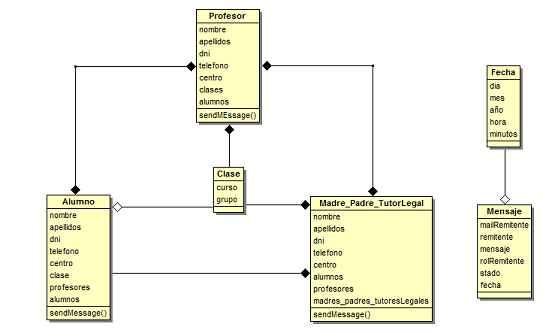
\includegraphics{CollegeAppDiagramaClases}
	\caption{Diagrama de Clases}
	\label{fig:ClassDiagram}
\end{figure}
 %Listo
	%
% ---------------------------------------------------
%
% Trabajo de Final de Grado:
% Author: Gonzalo Jesús García Martín <dracoyue@gmail.com>
% Capítulo:  Diagrama de actividades
% Fichero: ApendiceB_DiagramaActividades.tex
%
% ----------------------------------------------------
%

\cleardoublepage
\chapter{Diagrama de Actividades}
\label{chap:activitiesdiagram}

Se puede ver una imagen del diagrama de actividades:

\begin{figure}[h !]
	\centering
	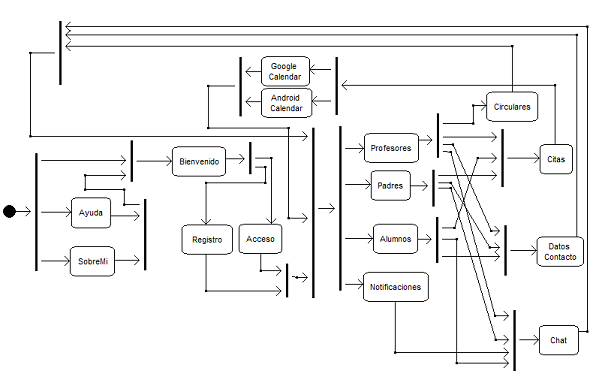
\includegraphics{CollegeAppDiagramaActividades}
	\caption{Diagrama de Actividades}
	\label{fig:ActivitiesDiagram}
\end{figure}

Cada uno de los nodos es una actividad, representando las flechas el acceso a otras actividades. Las barras verticales representan que desde múltiples actividades se pueden acceder a una o varias. %Listo
	%%
% ---------------------------------------------------
%
% Trabajo de Final de Grado:
% Author: Gonzalo Jesús García Martín <dracoyue@gmail.com>
% Capítulo:  Diagrama de actividades
% Fichero: ApendiceC_MapaActividades.tex
%
% ----------------------------------------------------
%

\cleardoublepage
\chapter{Secuencia de Actividades}
\label{chap:activitiesSecuence}

Se puede ver una imagen de la secuencia de actividades que sigue la aplicación:

\begin{figure}[h]
	\centering
	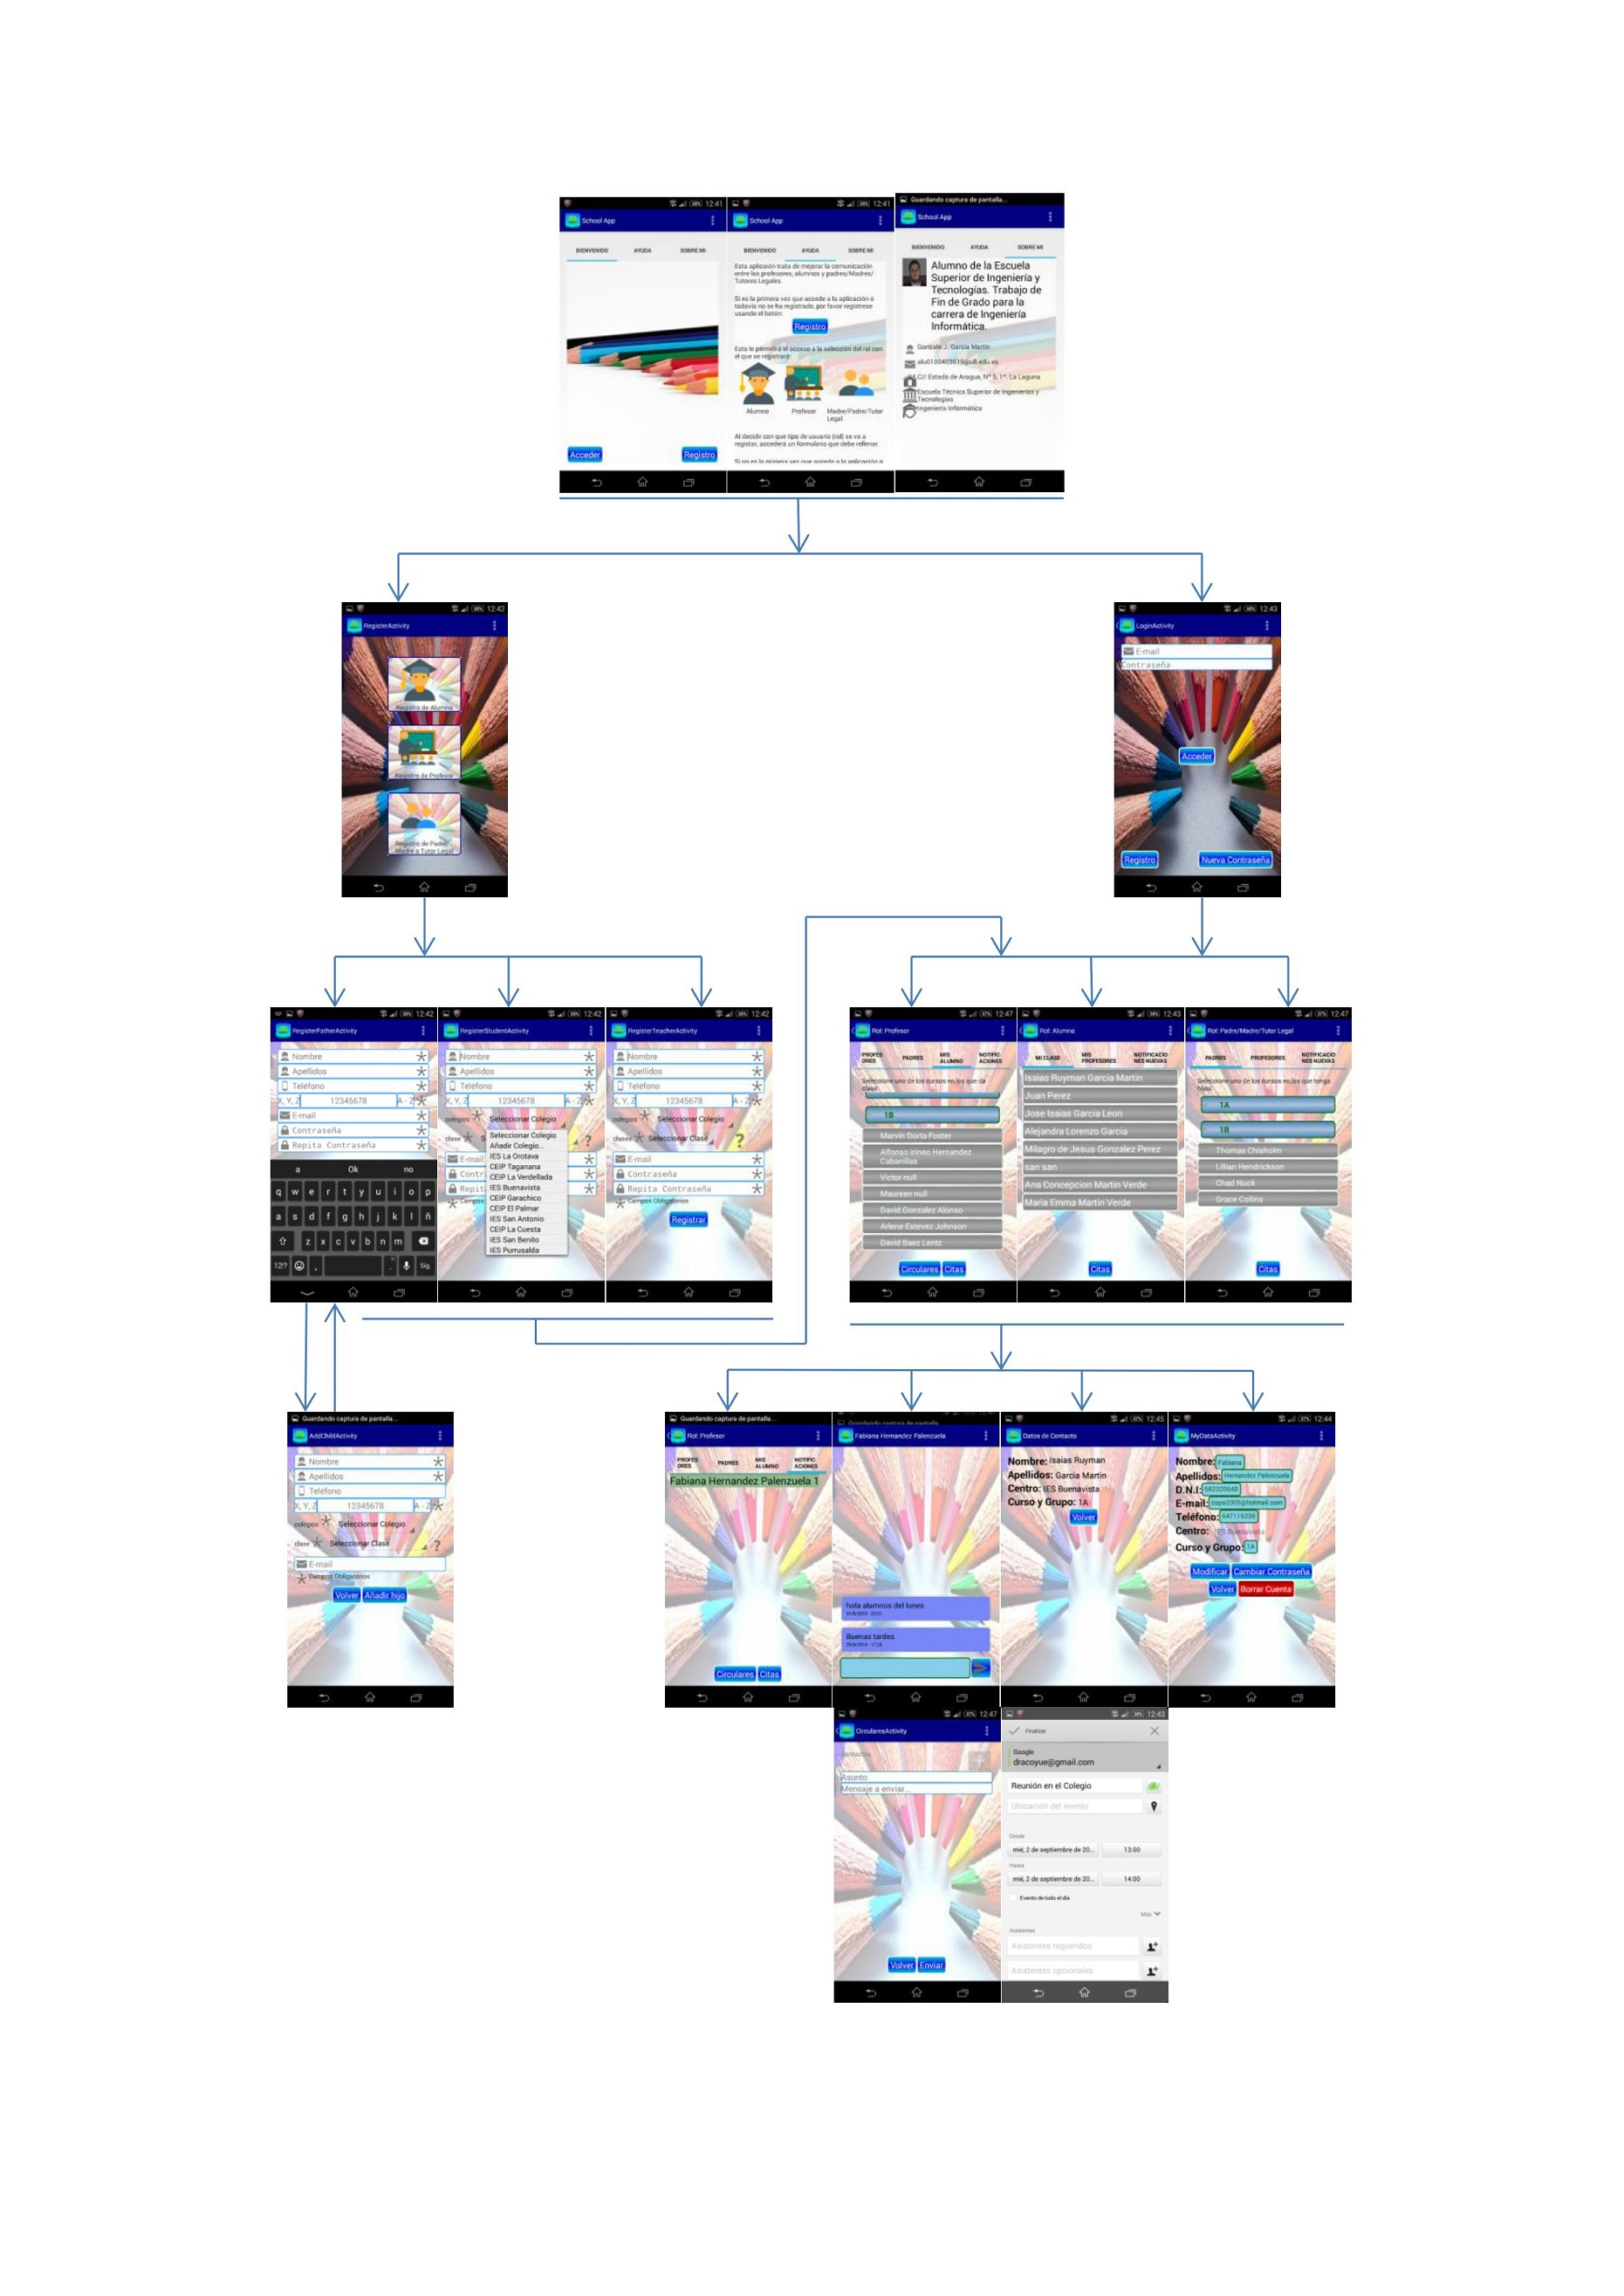
\includegraphics{mapaActividades}
	\caption{Secuencia de Actividades}
	\label{fig:ActivitiesSecuence}
\end{figure} %Listo
	
%%%%%%%%%%%%%%%%%%%%%%%%%%%%%%%%%%%%%%%%%%%%%%%%%%%%%%%%%%%%%%%%%%%%%%%%%%%%%%%%%%%%%%%%%%%%%%%%
	%Bibliografía
	\bibliographystyle{unsrt}
	\bibliography{Bibliografia/bibliography}
	
\end{document}
